% Options for packages loaded elsewhere
\PassOptionsToPackage{unicode}{hyperref}
\PassOptionsToPackage{hyphens}{url}
%
\documentclass[
]{article}
\usepackage{amsmath,amssymb}
\usepackage{iftex}
\ifPDFTeX
  \usepackage[T1]{fontenc}
  \usepackage[utf8]{inputenc}
  \usepackage{textcomp} % provide euro and other symbols
\else % if luatex or xetex
  \usepackage{unicode-math} % this also loads fontspec
  \defaultfontfeatures{Scale=MatchLowercase}
  \defaultfontfeatures[\rmfamily]{Ligatures=TeX,Scale=1}
\fi
\usepackage{lmodern}
\ifPDFTeX\else
  % xetex/luatex font selection
\fi
% Use upquote if available, for straight quotes in verbatim environments
\IfFileExists{upquote.sty}{\usepackage{upquote}}{}
\IfFileExists{microtype.sty}{% use microtype if available
  \usepackage[]{microtype}
  \UseMicrotypeSet[protrusion]{basicmath} % disable protrusion for tt fonts
}{}
\makeatletter
\@ifundefined{KOMAClassName}{% if non-KOMA class
  \IfFileExists{parskip.sty}{%
    \usepackage{parskip}
  }{% else
    \setlength{\parindent}{0pt}
    \setlength{\parskip}{6pt plus 2pt minus 1pt}}
}{% if KOMA class
  \KOMAoptions{parskip=half}}
\makeatother
\usepackage{xcolor}
\usepackage[margin=1in]{geometry}
\usepackage{graphicx}
\makeatletter
\newsavebox\pandoc@box
\newcommand*\pandocbounded[1]{% scales image to fit in text height/width
  \sbox\pandoc@box{#1}%
  \Gscale@div\@tempa{\textheight}{\dimexpr\ht\pandoc@box+\dp\pandoc@box\relax}%
  \Gscale@div\@tempb{\linewidth}{\wd\pandoc@box}%
  \ifdim\@tempb\p@<\@tempa\p@\let\@tempa\@tempb\fi% select the smaller of both
  \ifdim\@tempa\p@<\p@\scalebox{\@tempa}{\usebox\pandoc@box}%
  \else\usebox{\pandoc@box}%
  \fi%
}
% Set default figure placement to htbp
\def\fps@figure{htbp}
\makeatother
\setlength{\emergencystretch}{3em} % prevent overfull lines
\providecommand{\tightlist}{%
  \setlength{\itemsep}{0pt}\setlength{\parskip}{0pt}}
\setcounter{secnumdepth}{-\maxdimen} % remove section numbering
\ifLuaTeX
\usepackage[bidi=basic]{babel}
\else
\usepackage[bidi=default]{babel}
\fi
\babelprovide[main,import]{french}
% get rid of language-specific shorthands (see #6817):
\let\LanguageShortHands\languageshorthands
\def\languageshorthands#1{}
\usepackage{bookmark}
\IfFileExists{xurl.sty}{\usepackage{xurl}}{} % add URL line breaks if available
\urlstyle{same}
\hypersetup{
  pdftitle={Synthèse des comptes trimestriels : comptes d'agents},
  pdfauthor={@statjunior},
  pdflang={fr-FR},
  hidelinks,
  pdfcreator={LaTeX via pandoc}}

\title{Synthèse des comptes trimestriels : comptes d'agents}
\usepackage{etoolbox}
\makeatletter
\providecommand{\subtitle}[1]{% add subtitle to \maketitle
  \apptocmd{\@title}{\par {\large #1 \par}}{}{}
}
\makeatother
\subtitle{Résultats détaillés des \emph{Comptes Nationaux Trimestriels}
au 1er trimestre 2024.}
\author{@statjunior}
\date{30 juillet 2024}

\begin{document}
\maketitle

\section{Présentation}\label{pruxe9sentation}

Ce rapport \emph{RMarkdown} présente les résultats détaillés des comptes
des secteurs institutionnels (ménages, entreprises, administrations
publiques, reste du monde) au 1er trimestre 2024.

Le rapport présente successivement les grands indicateurs
macroéconomiques à retenir pour chaque agent économique.

Pour les ménages, on présente d'abord le revenu disponible brut et les
prix à la consommation en comptabilité nationale afin d'en déduire le
pouvoir d'achat des ménages. Le pouvoir d'achat des ménages est un
indicateur macroéconomique qui ne tient pas compte de la taille des
ménages et des économies d'échelle. C'est pourquoi on présente également
le pouvoir d'achat par unité de consommation (UC). Le pouvoir d'achat
des ménages par UC tient compte de la croissance de la population et des
économies ou d'échelle liées à la vie sous un même toit. Enfin, on
présente les contributions à l'évolution du pouvoir d'achat afin de
distinguer une variation liée aux revenus du travail, à la fiscalité,
aux prestations ou aux revenus du capital.

Pour les entreprises, on s'intéresse principalement aux sociétés non
financières (SNF). On présente tout d'abord leur taux de marge et leur
taux d'investissement sur longue période. Puis, on décompose les
contributions de l'évolution du taux de marge depuis 2019.

On s'intéresse ensuite aux comptes des administrations publiques (APU).
On présente l'évolution des recettes et des dépenses publiques sur
longue période ainsi que l'élasticité des recettes publiques par rapport
au PIB. On distingue ensuite l'évolution des dépenses par grande
composante. Enfin, on présente l'évolution du déficit public sur longue
période ainsi que la charge d'intérêt de la dette.

Enfin, on présente la situation de financement de l'économie française
vis à vis du reste du monde.

Ce rapport a été compilé automatiquement avec le logiciel \texttt{R}, le
30 juillet 2024 à 10 heures et 11 minutes. Les potentielles erreurs
présentes dans ce document relèvent uniquement de la responsabilité de
Statjunior.

Le code source permettant de générer ce document est disponible sur Git
\href{https://github.com/statjunior/Statjunior/tree/main/Conjoncture\%20-\%20comptes\%20trimestriels/}{en
cliquant ici}.

\section{Compte des ménages}\label{compte-des-muxe9nages}

\subsection{Revenu disponible brut et pouvoir d'achat depuis
2000}\label{revenu-disponible-brut-et-pouvoir-dachat-depuis-2000}

\pandocbounded{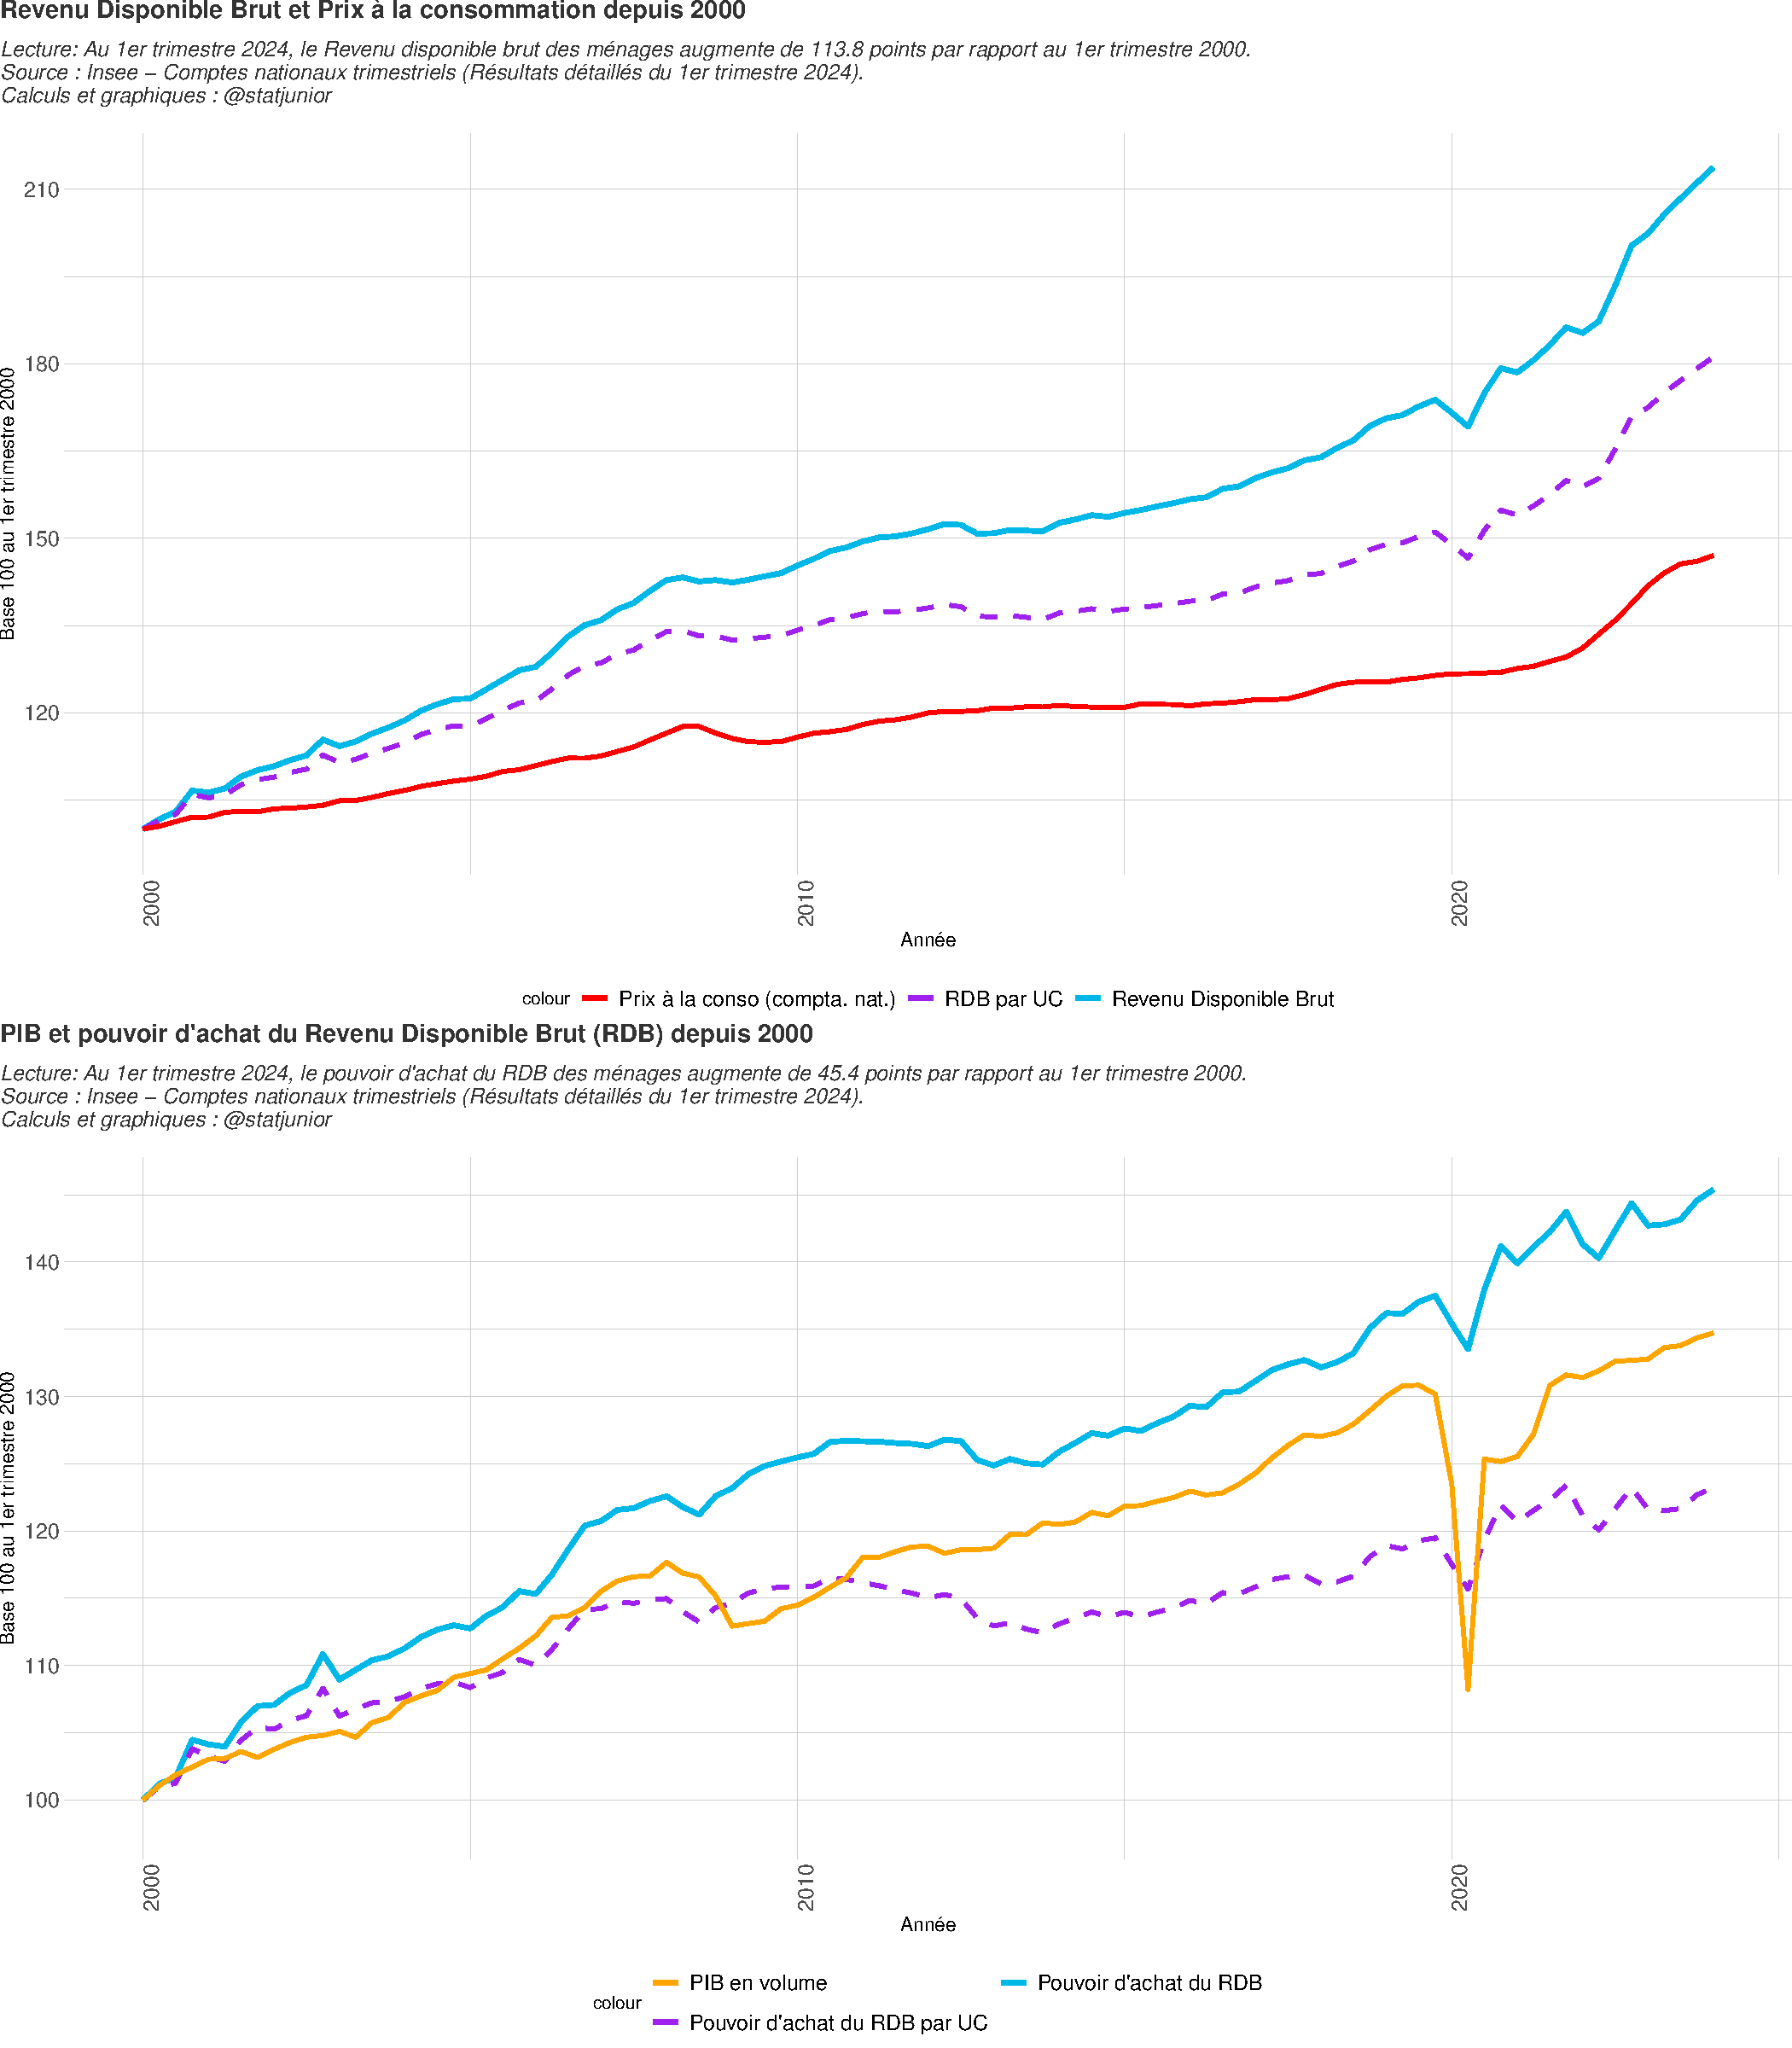
\includegraphics[keepaspectratio]{rapport_pdf_csi_files/figure-latex/unnamed-chunk-2-1.pdf}}

\subsection{Revenu disponible brut et pouvoir d'achat depuis
2019}\label{revenu-disponible-brut-et-pouvoir-dachat-depuis-2019}

\pandocbounded{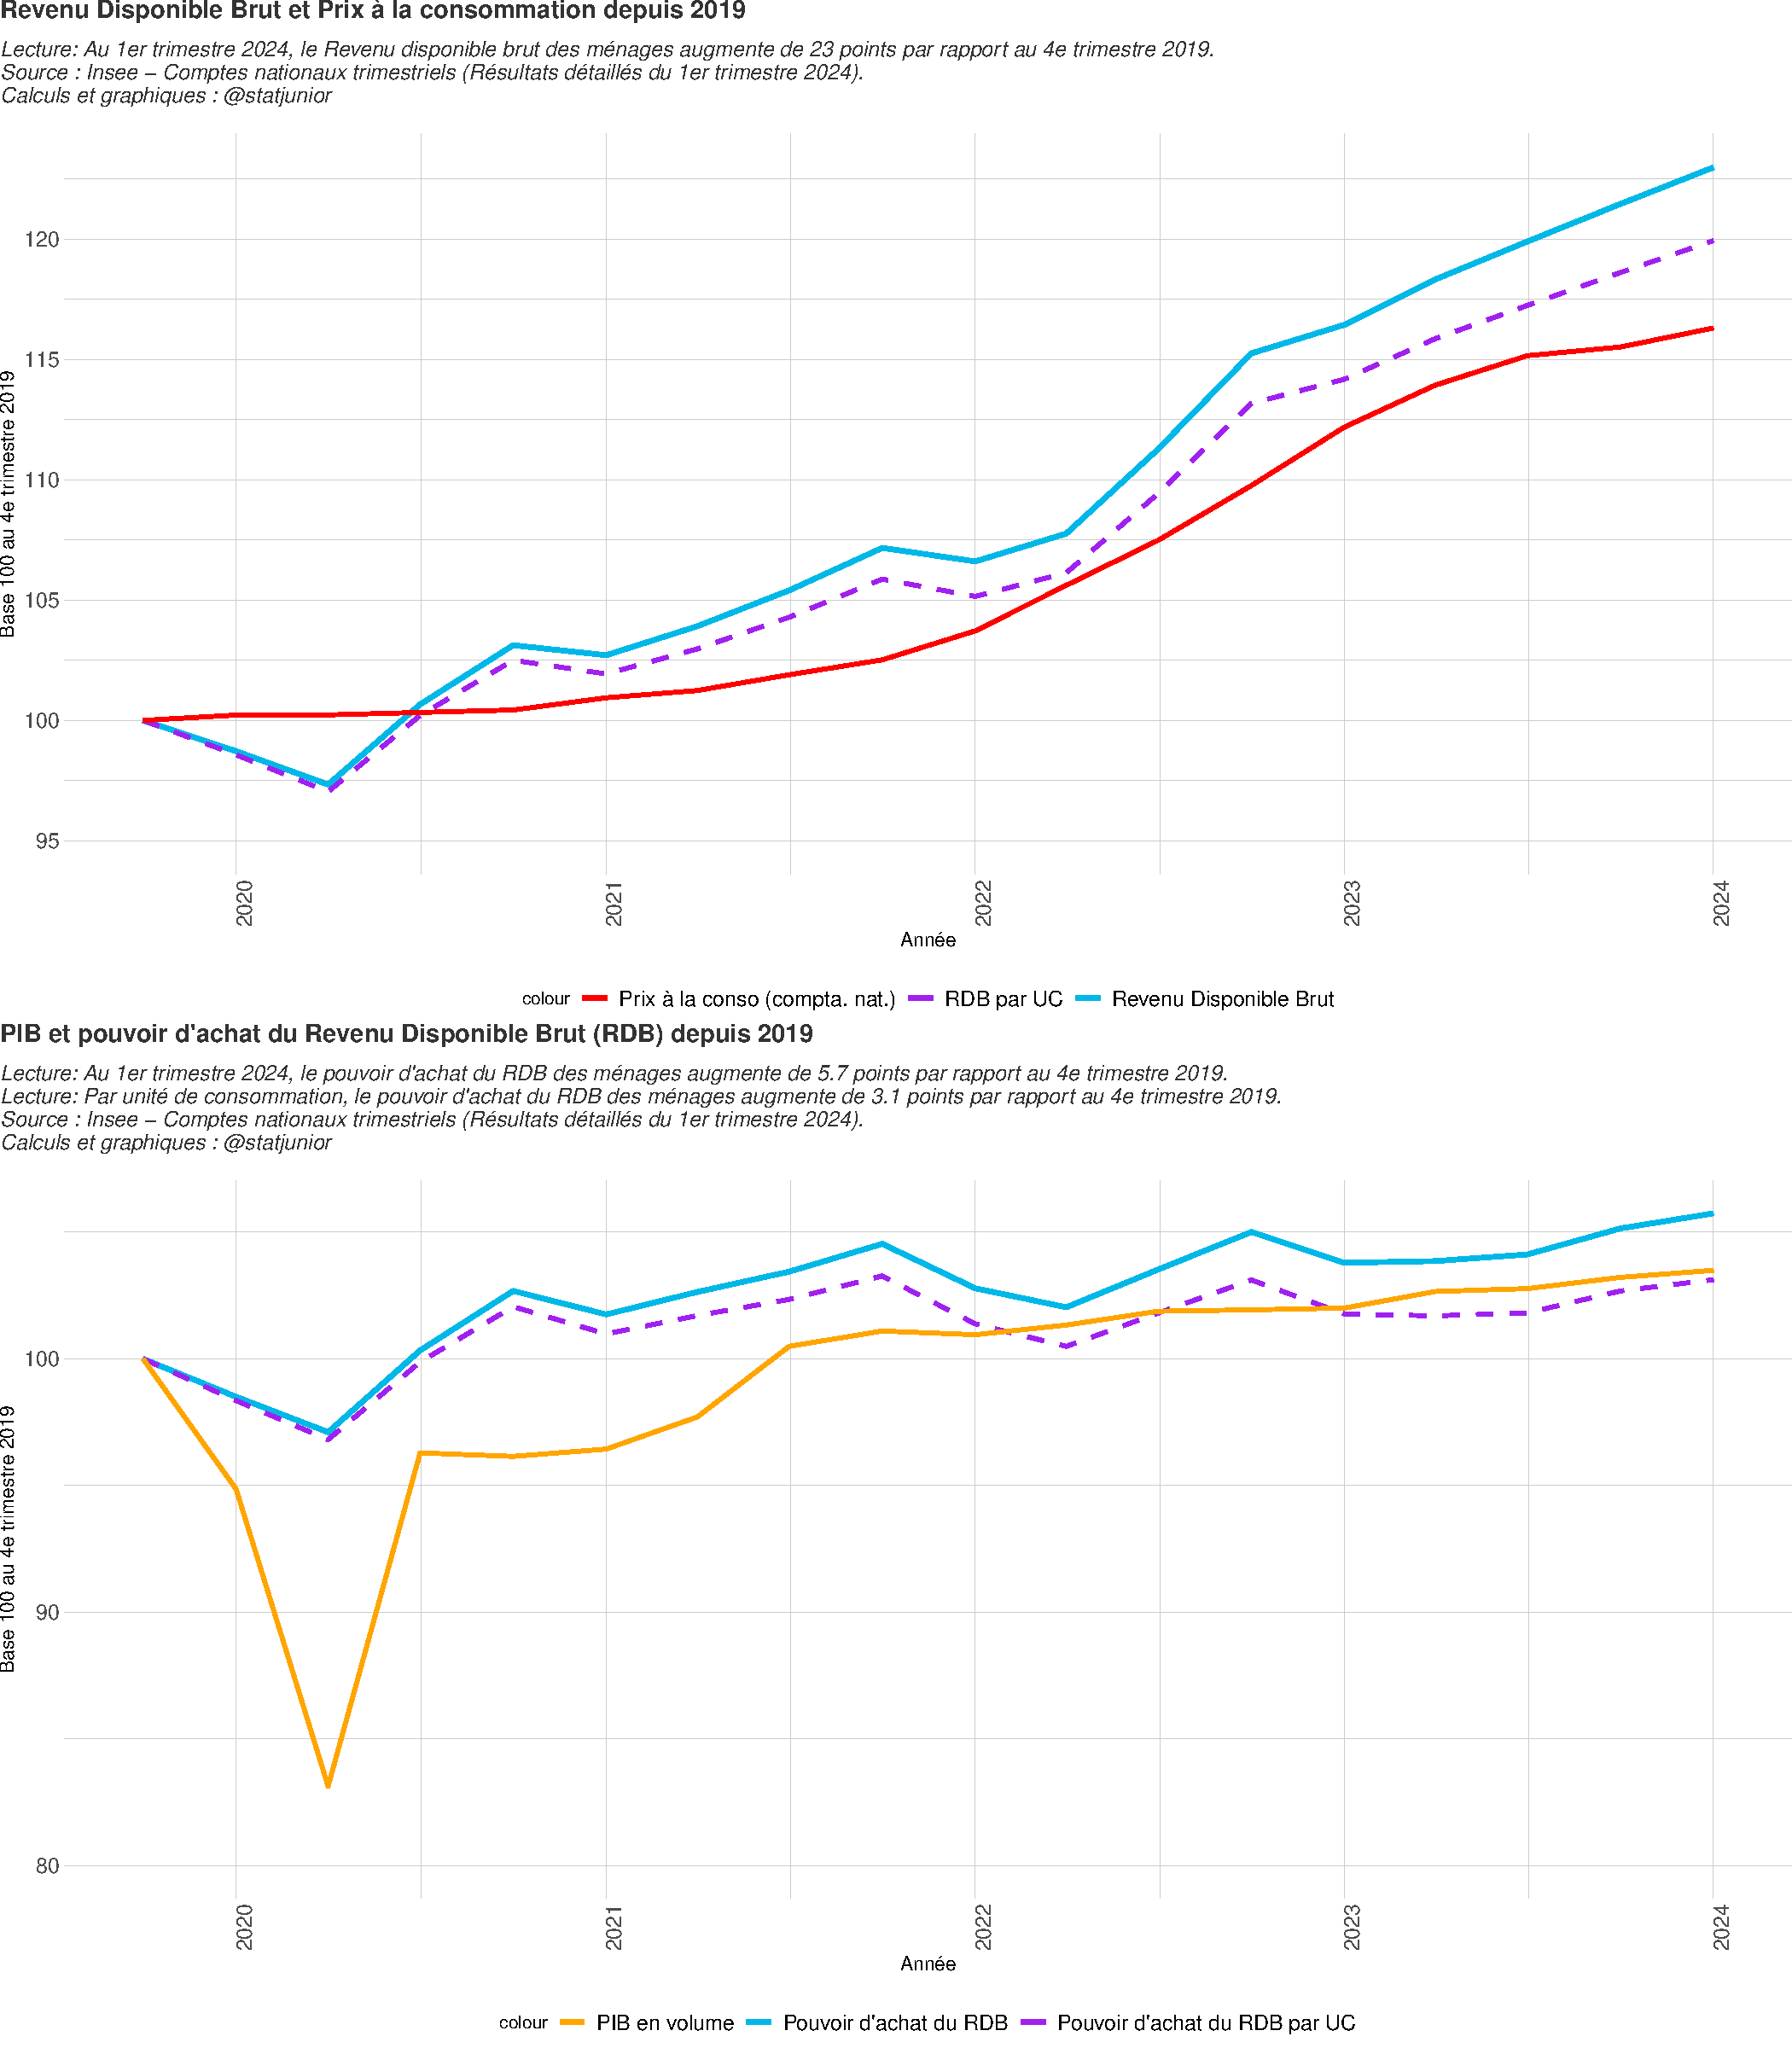
\includegraphics[keepaspectratio]{rapport_pdf_csi_files/figure-latex/unnamed-chunk-3-1.pdf}}

\subsection{Décomposition de l'évolution du pouvoir d'achat des ménages
depuis
2019}\label{duxe9composition-de-luxe9volution-du-pouvoir-dachat-des-muxe9nages-depuis-2019}

\pandocbounded{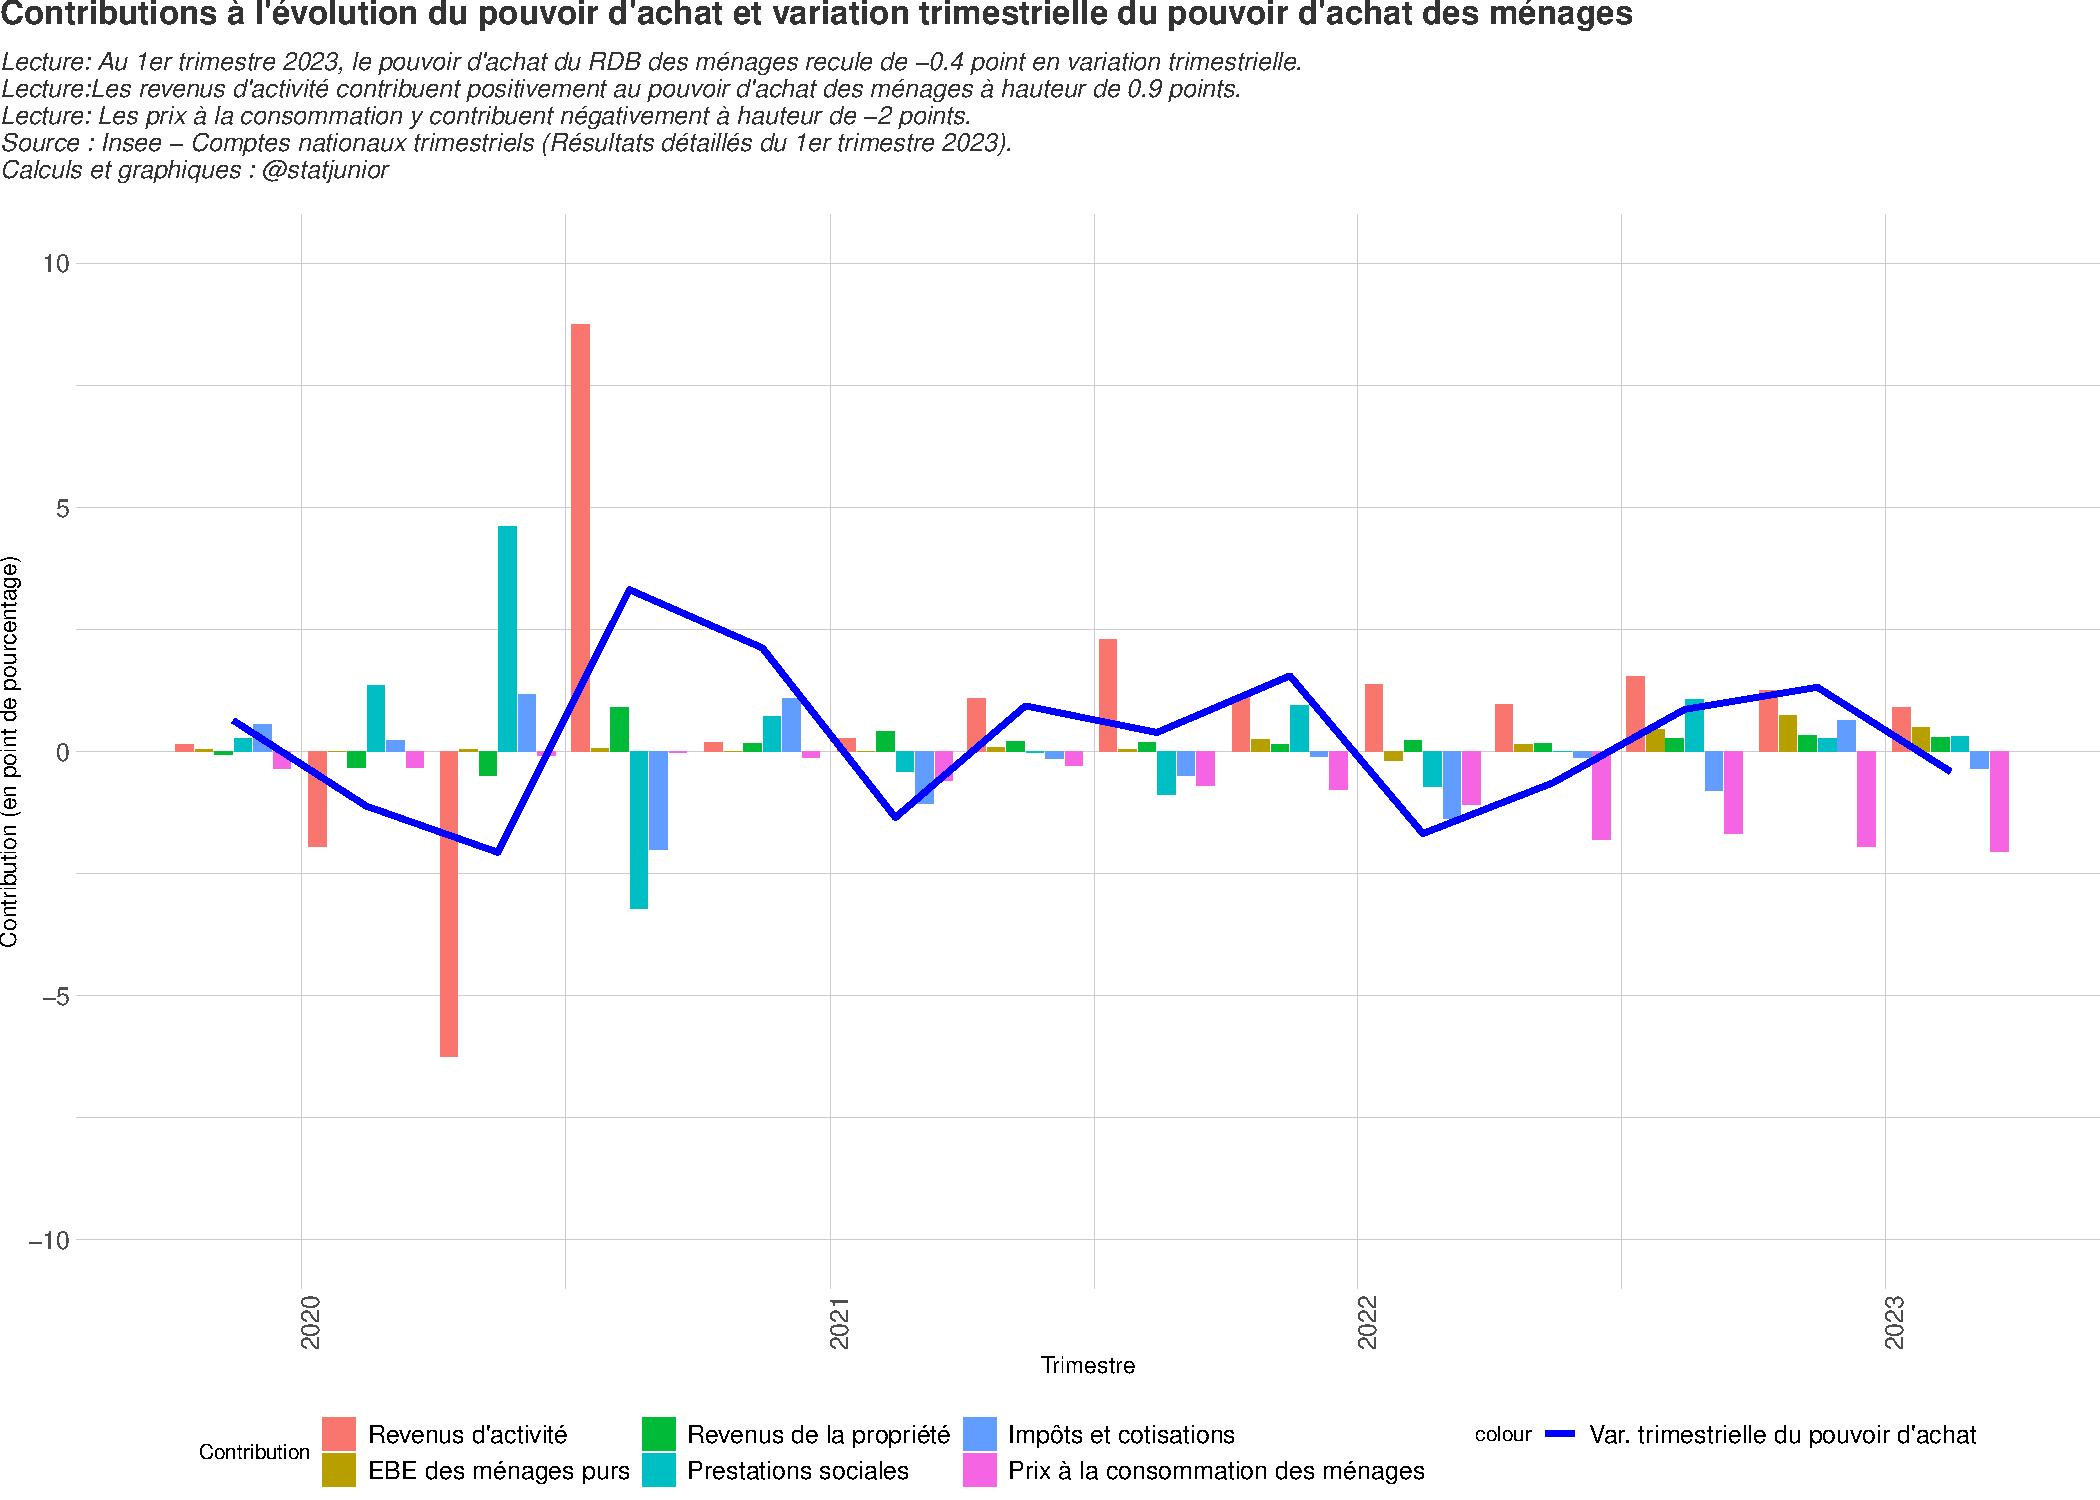
\includegraphics[keepaspectratio]{rapport_pdf_csi_files/figure-latex/unnamed-chunk-4-1.pdf}}

\subsection{Taux d'épargne des
ménages}\label{taux-duxe9pargne-des-muxe9nages}

\pandocbounded{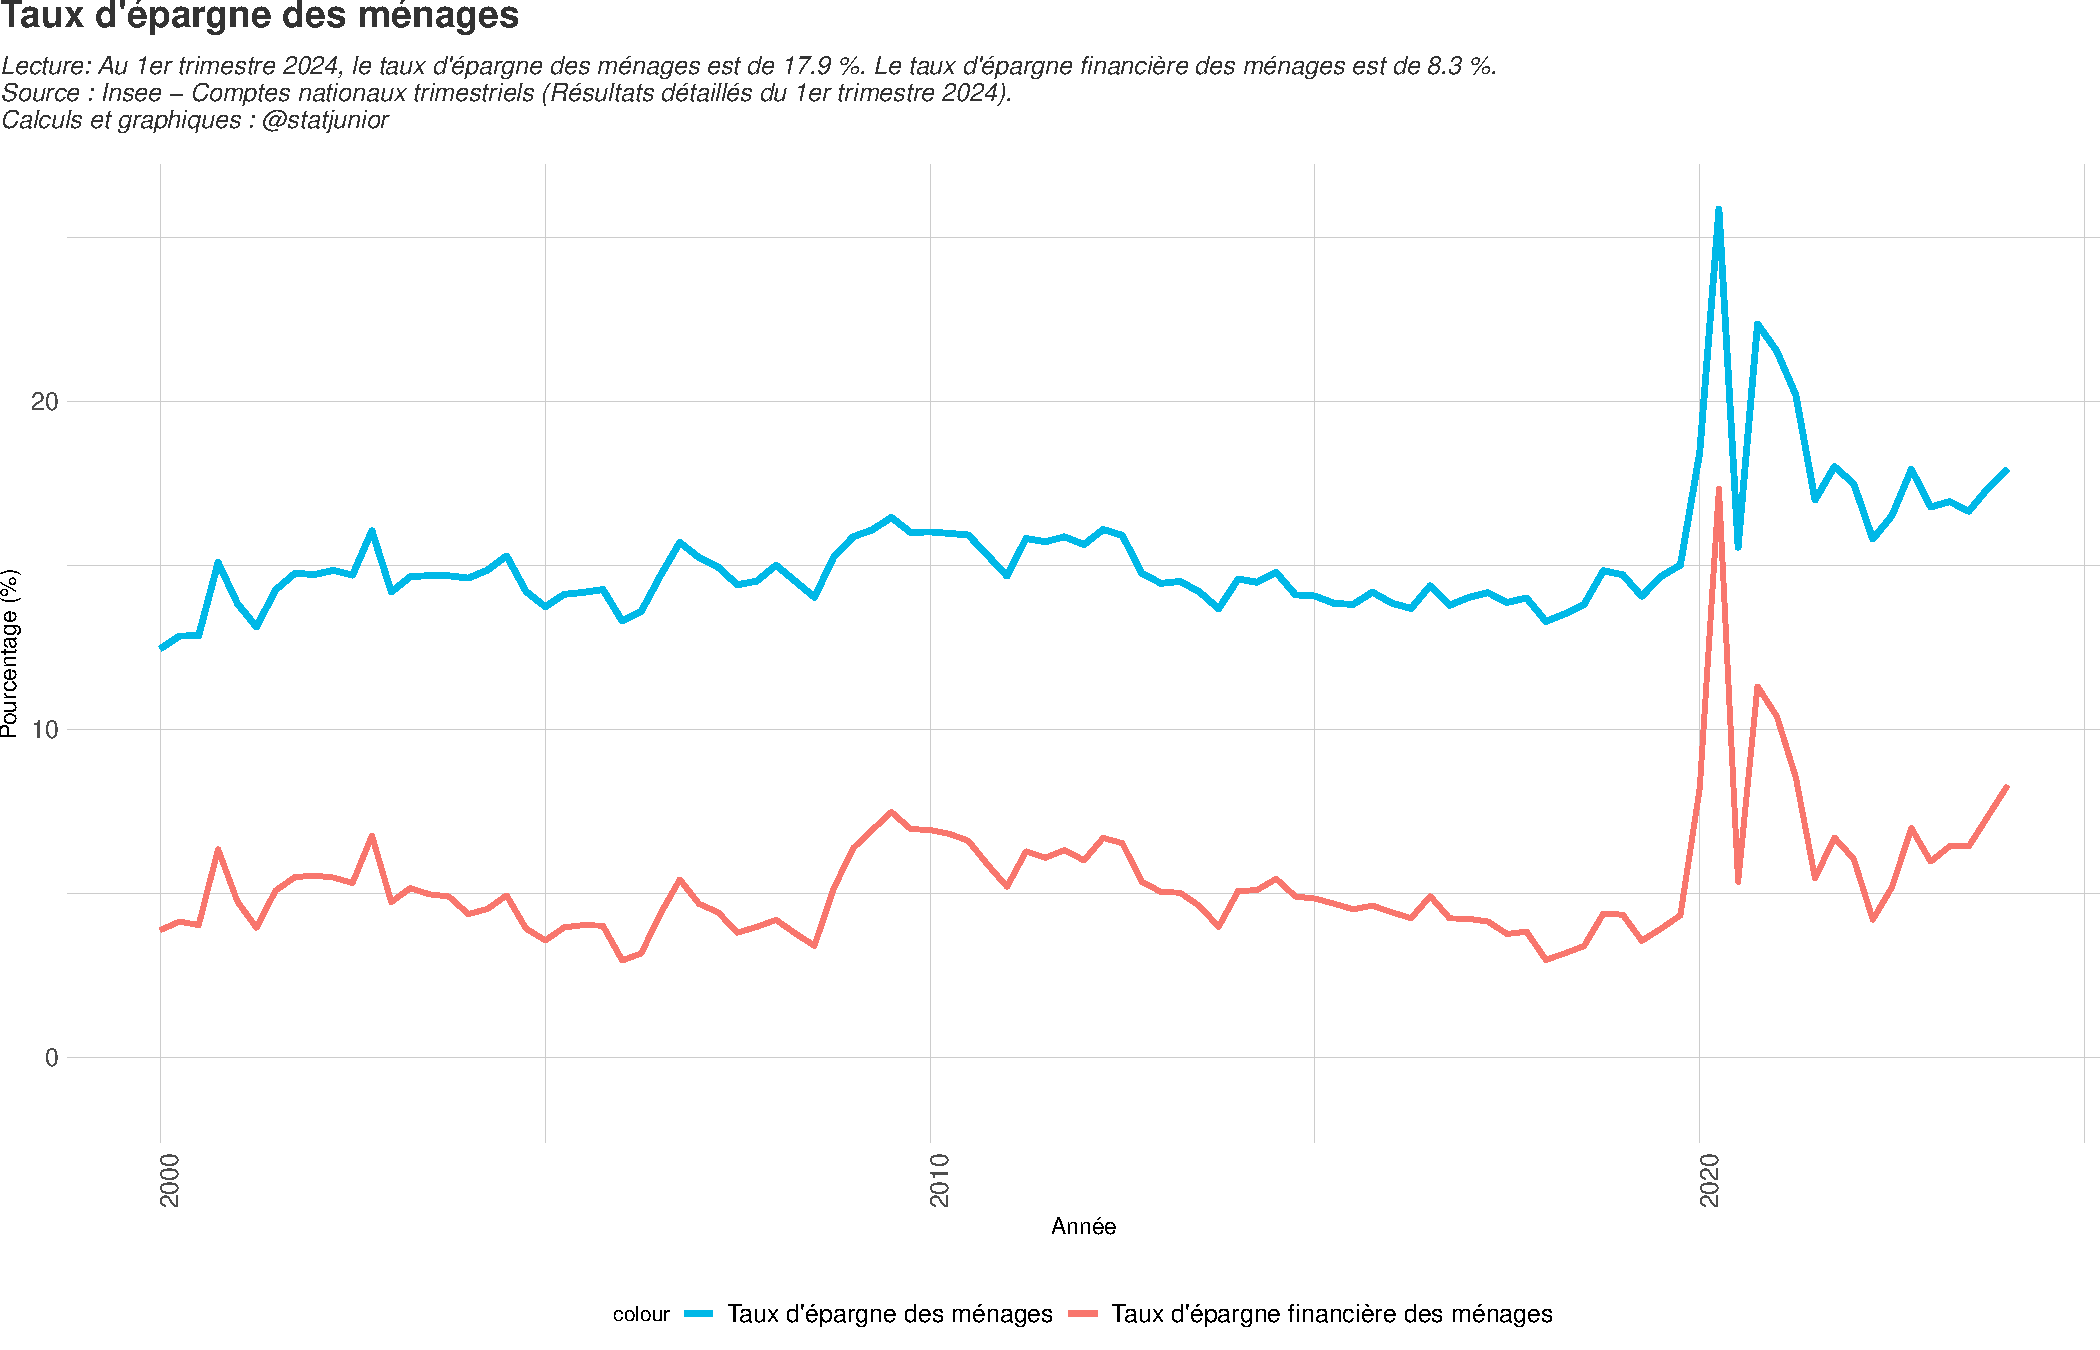
\includegraphics[keepaspectratio]{rapport_pdf_csi_files/figure-latex/unnamed-chunk-5-1.pdf}}

\newpage

\section{Compte des sociétés non financières
(SNF)}\label{compte-des-sociuxe9tuxe9s-non-financiuxe8res-snf}

\subsection{Taux de marge et taux d'investissement des SNF sur longue
période}\label{taux-de-marge-et-taux-dinvestissement-des-snf-sur-longue-puxe9riode}

\pandocbounded{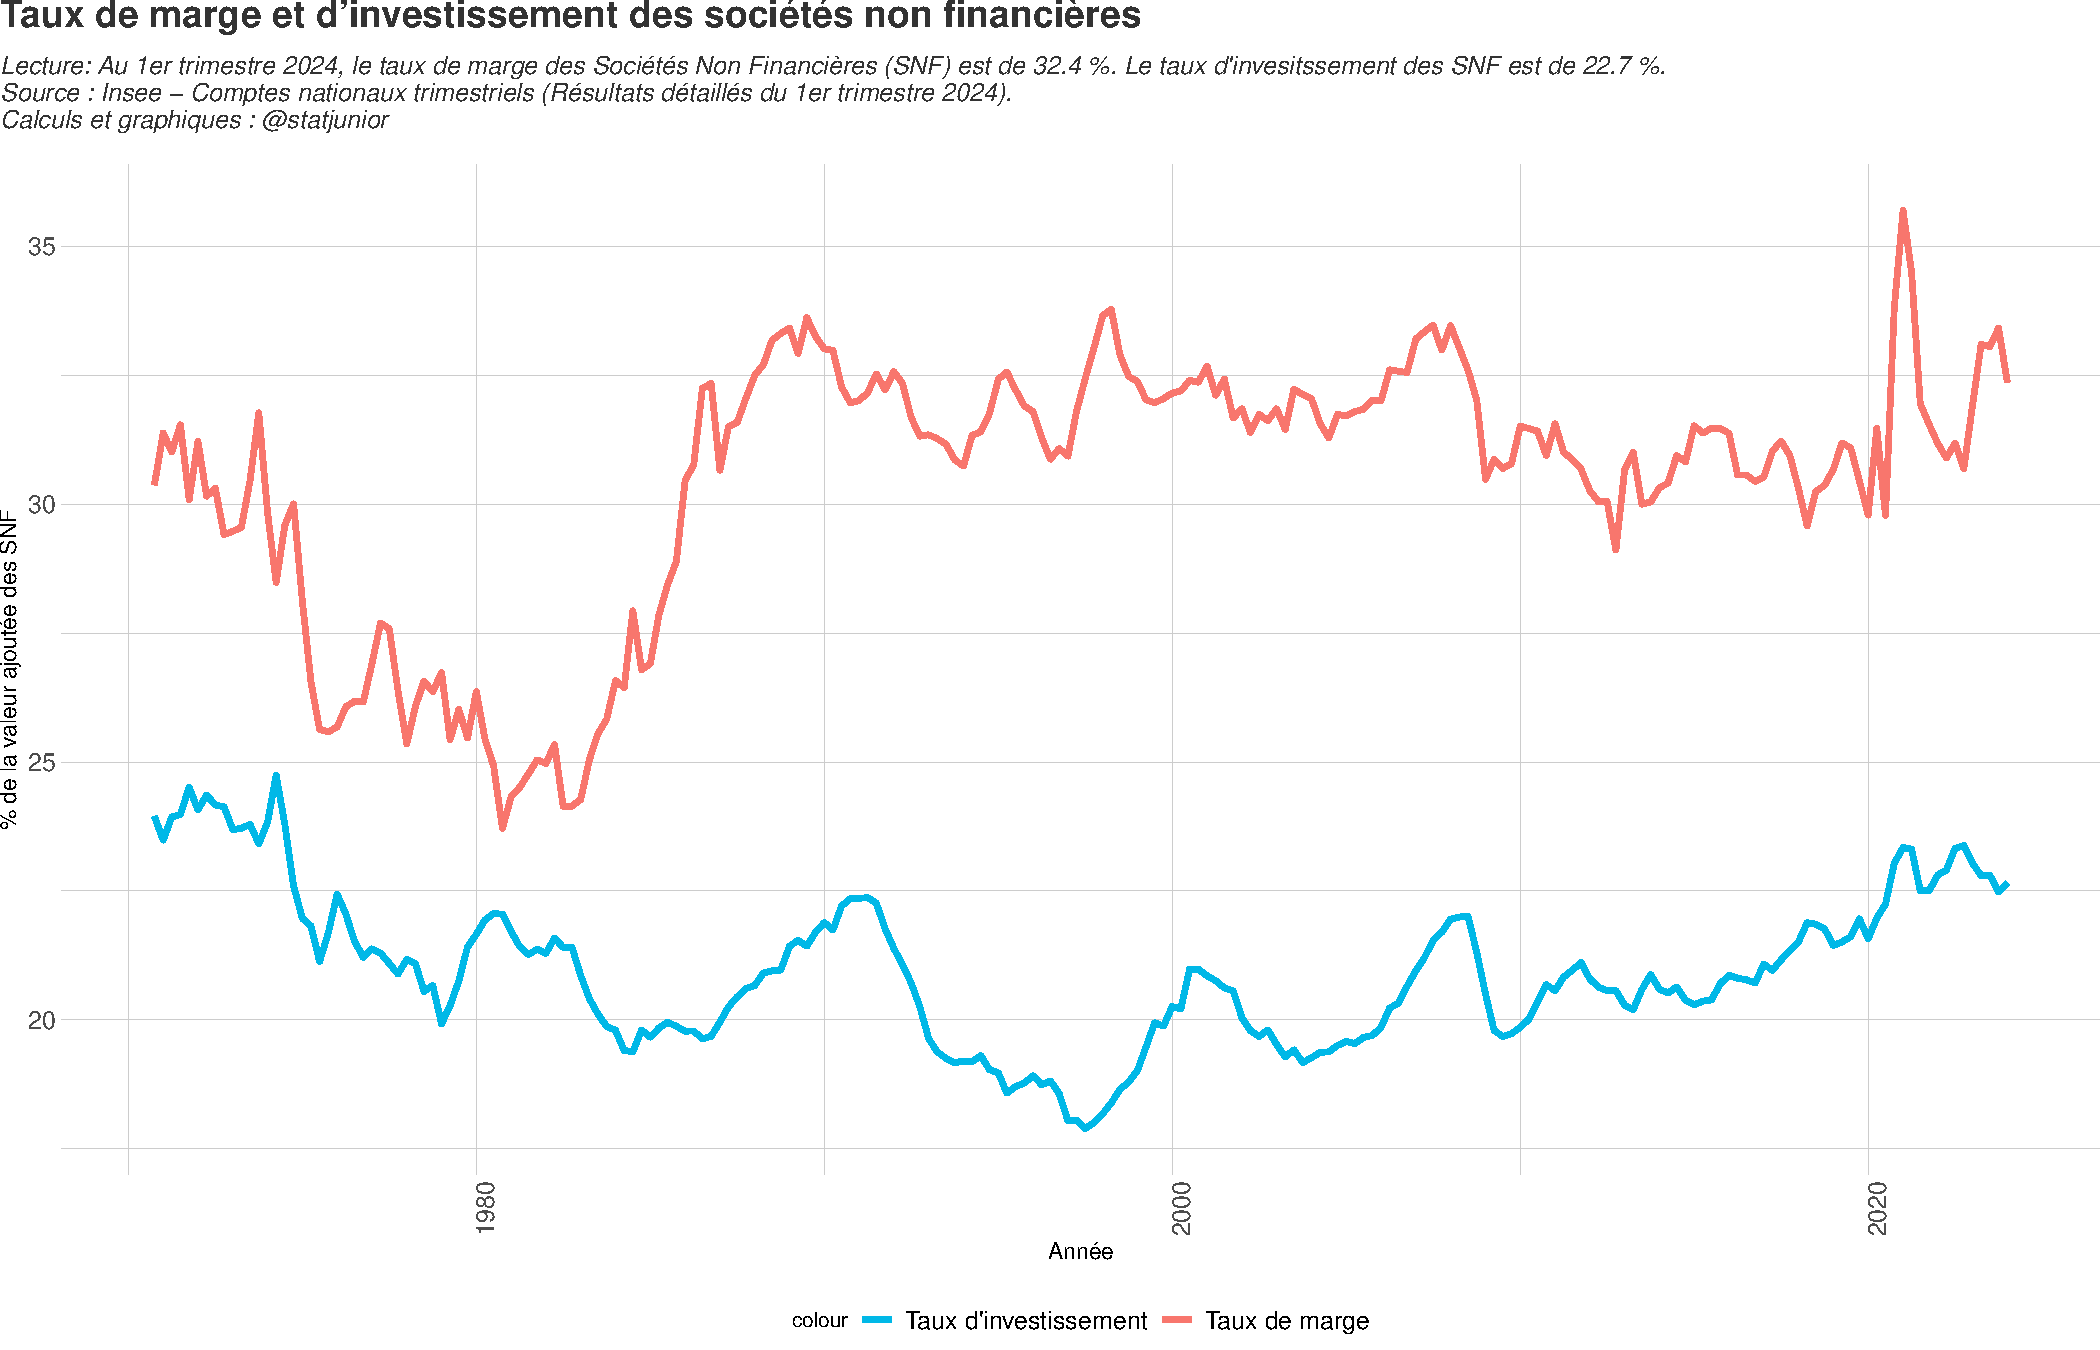
\includegraphics[keepaspectratio]{rapport_pdf_csi_files/figure-latex/unnamed-chunk-6-1.pdf}}

\subsection{Décomposition du taux des marges des SNF depuis
2018}\label{duxe9composition-du-taux-des-marges-des-snf-depuis-2018}

\pandocbounded{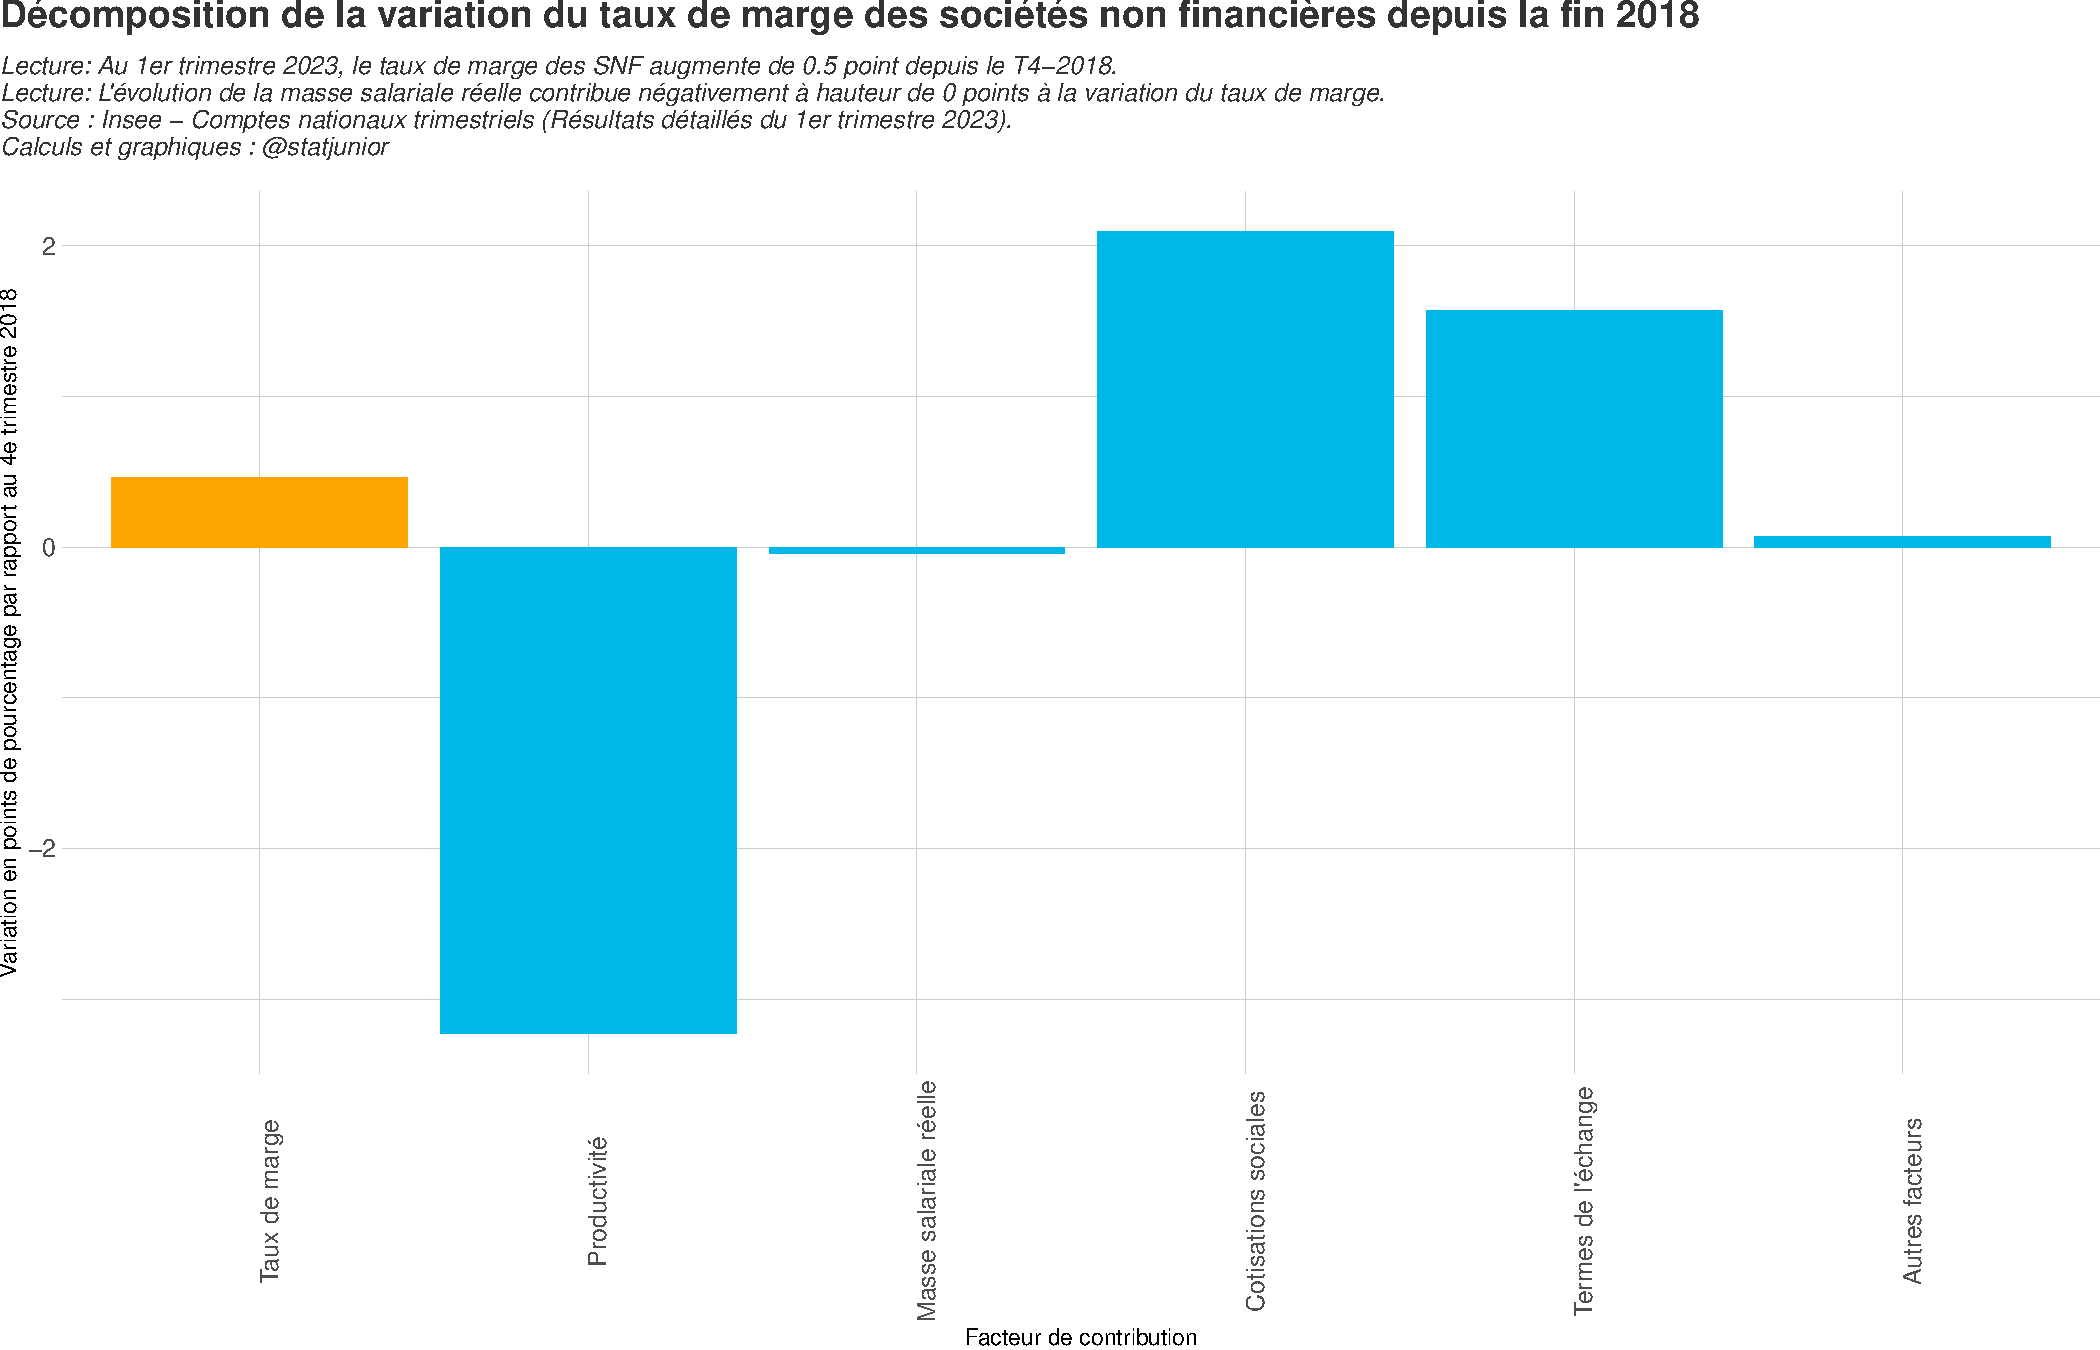
\includegraphics[keepaspectratio]{rapport_pdf_csi_files/figure-latex/unnamed-chunk-7-1.pdf}}

\newpage

\section{Comptes des administrations publiques
(APU)}\label{comptes-des-administrations-publiques-apu}

\subsection{Part des recettes et des dépenses des
APU}\label{part-des-recettes-et-des-duxe9penses-des-apu}

\pandocbounded{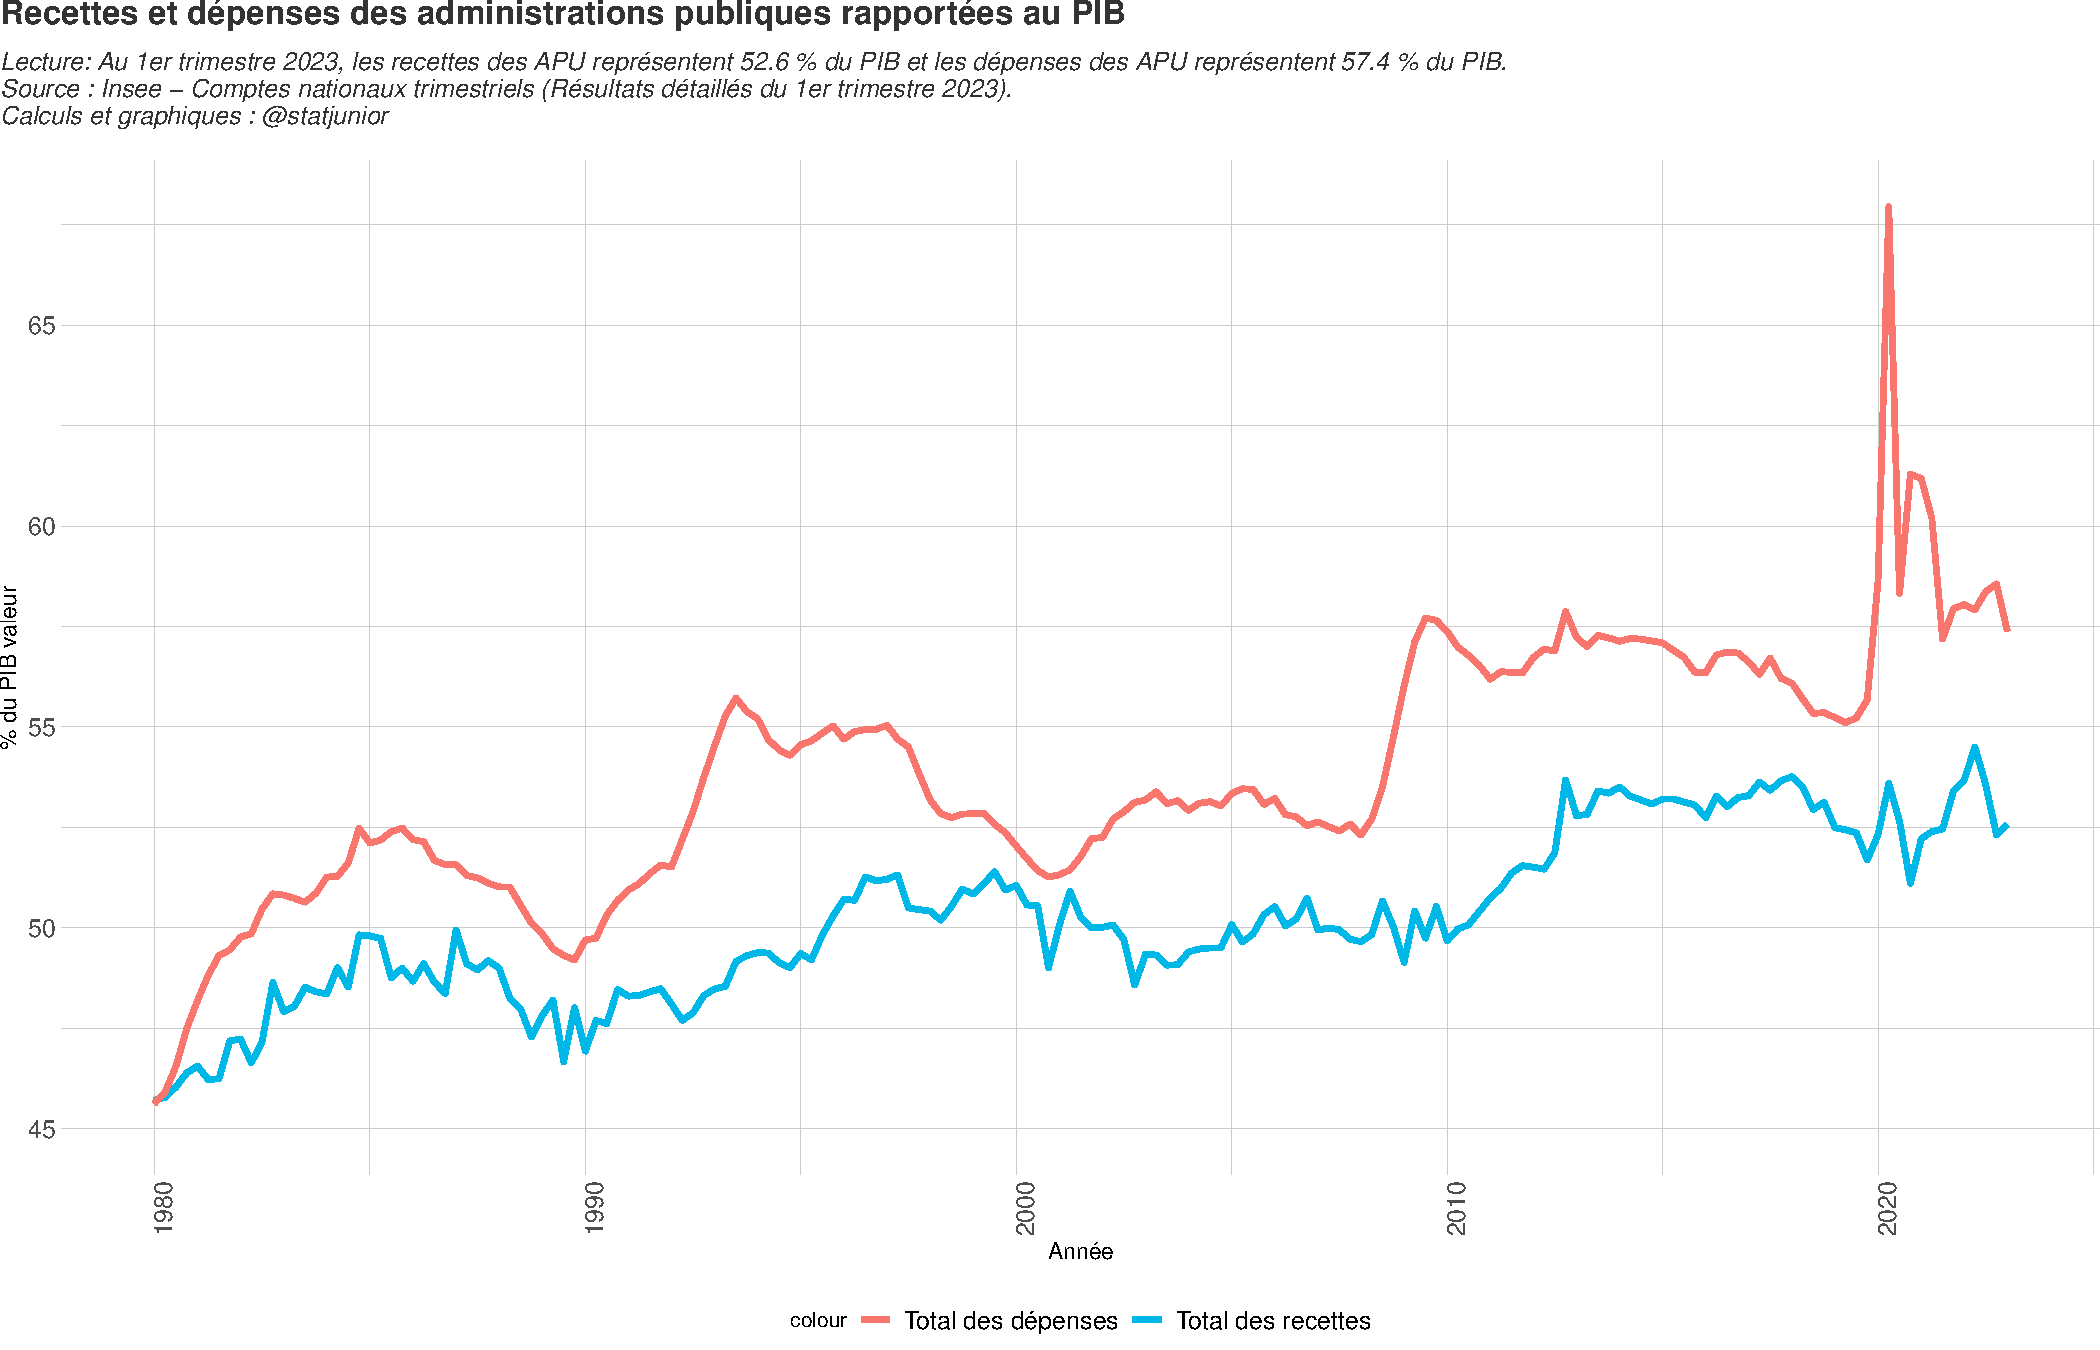
\includegraphics[keepaspectratio]{rapport_pdf_csi_files/figure-latex/unnamed-chunk-9-1.pdf}}

\subsection{Prélèvements obligatoires en part du
PIB}\label{pruxe9luxe8vements-obligatoires-en-part-du-pib}

\pandocbounded{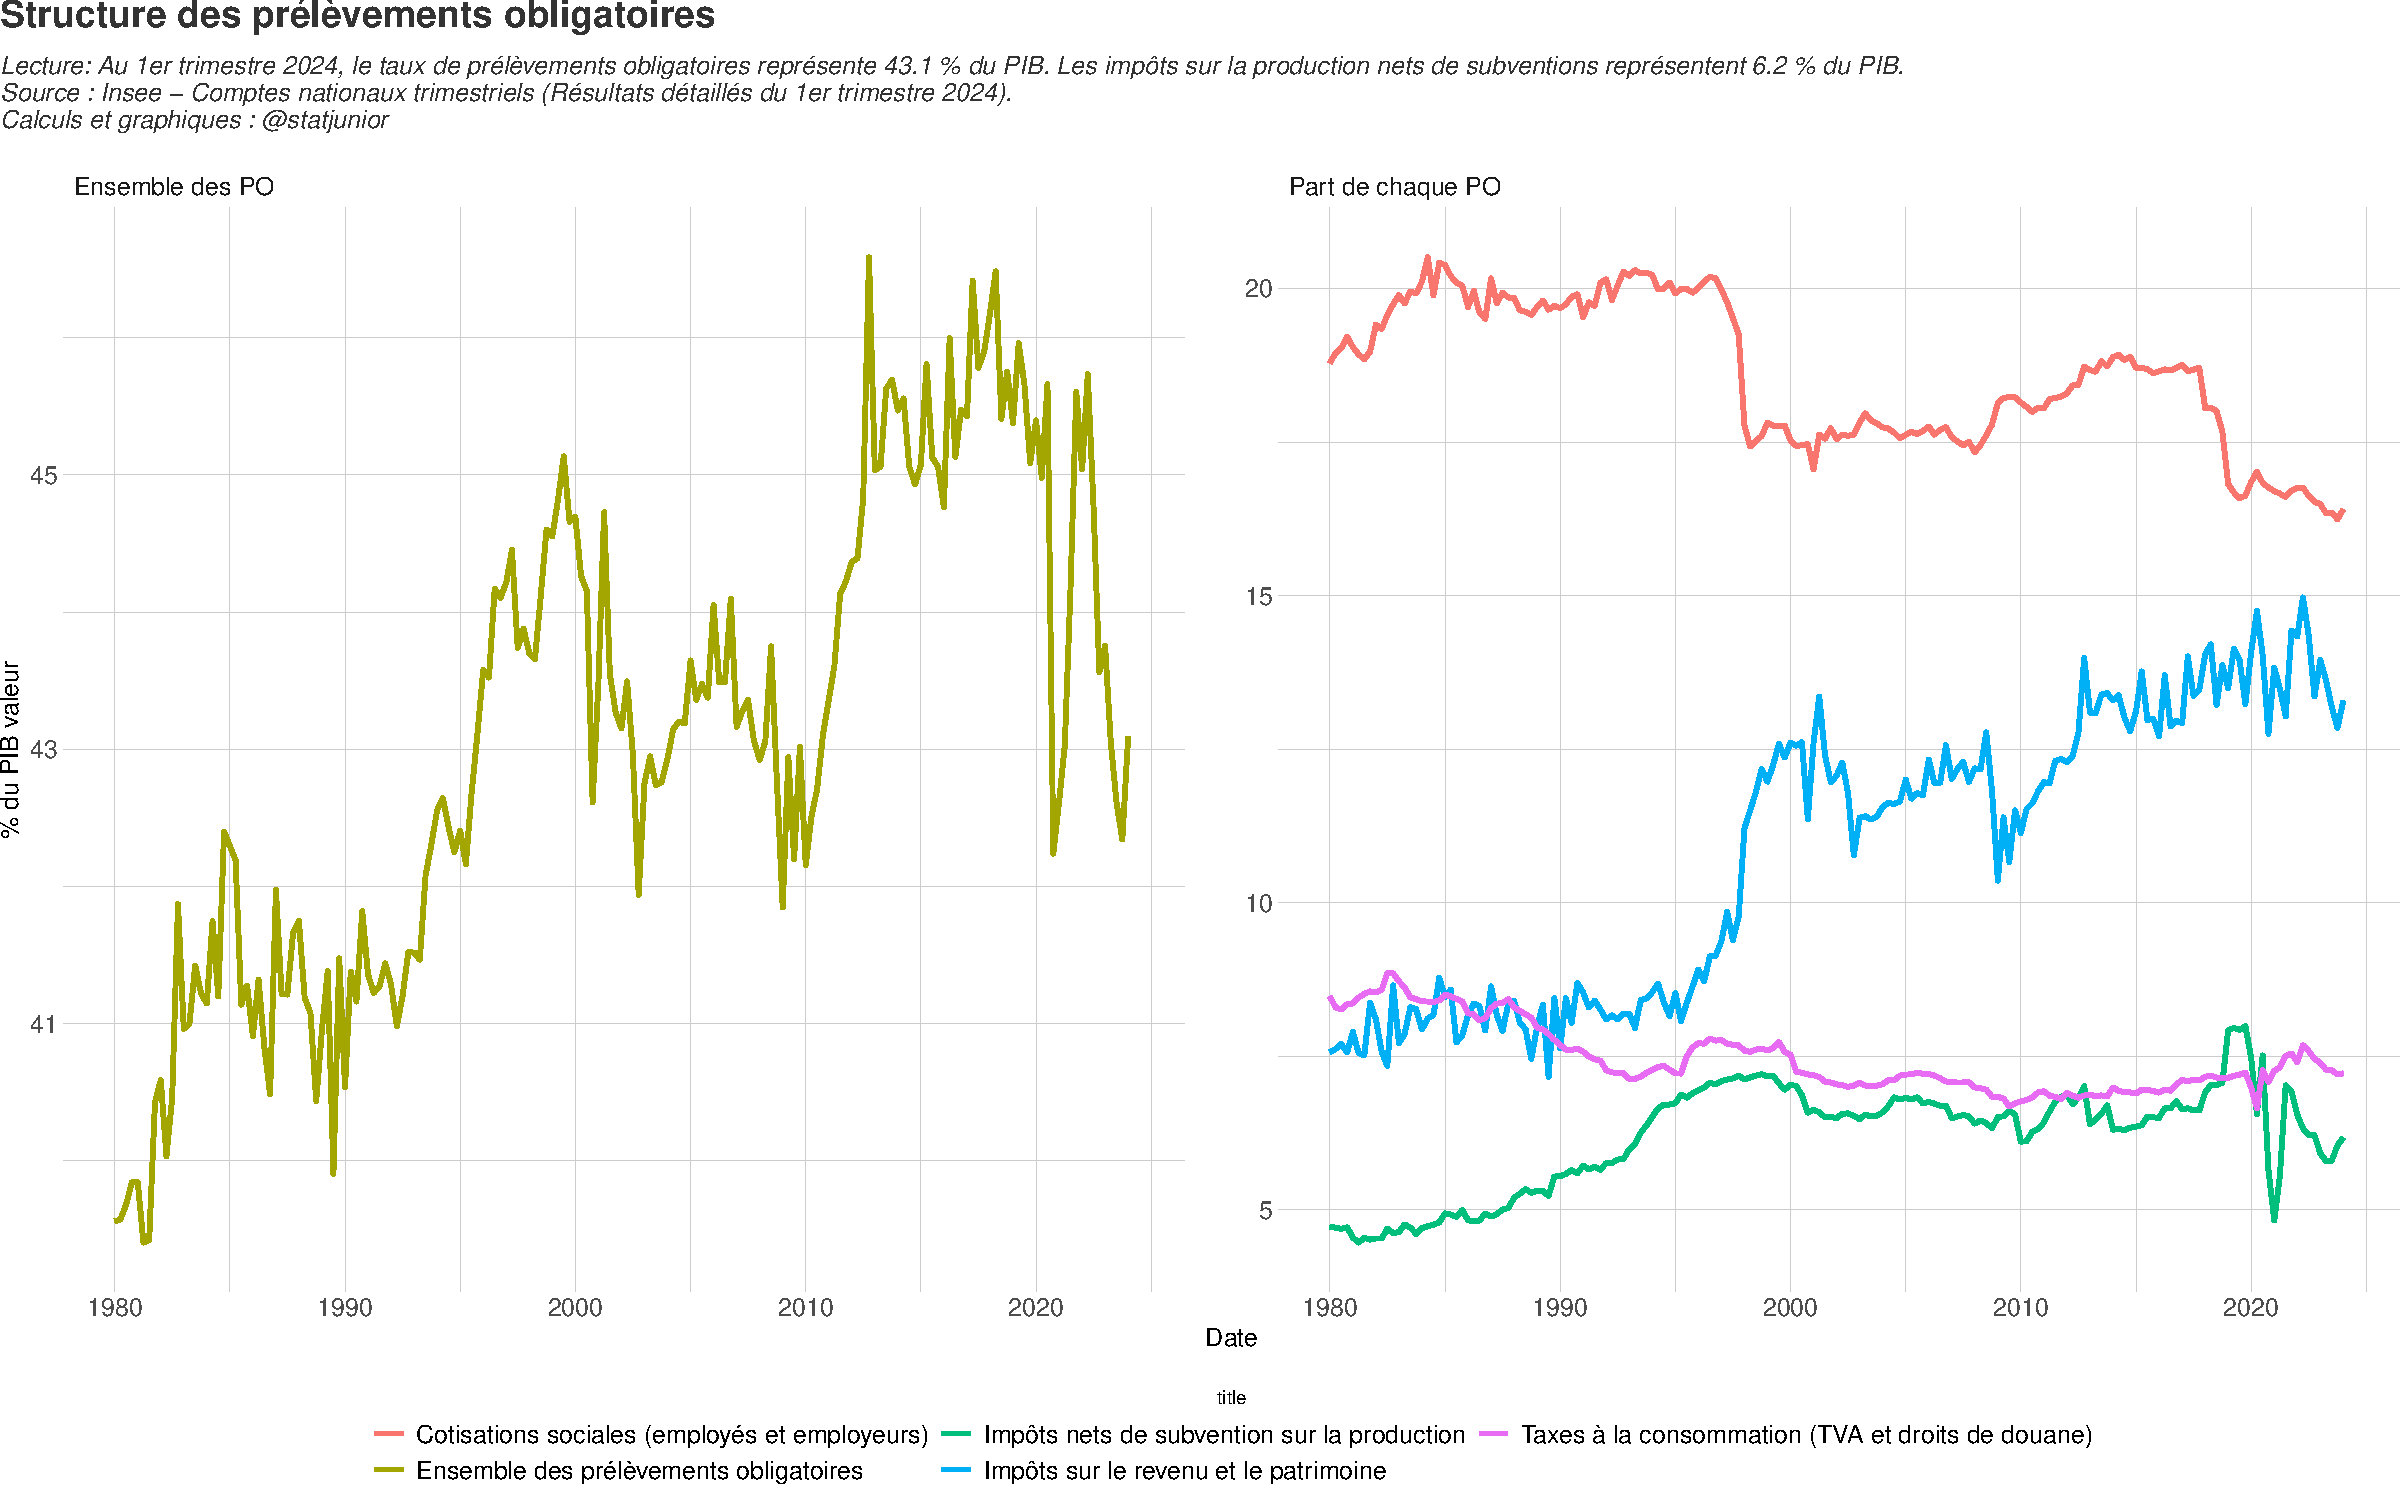
\includegraphics[keepaspectratio]{rapport_pdf_csi_files/figure-latex/unnamed-chunk-10-1.pdf}}

\subsection{Structure des prélèvements
obligatoires}\label{structure-des-pruxe9luxe8vements-obligatoires}

\pandocbounded{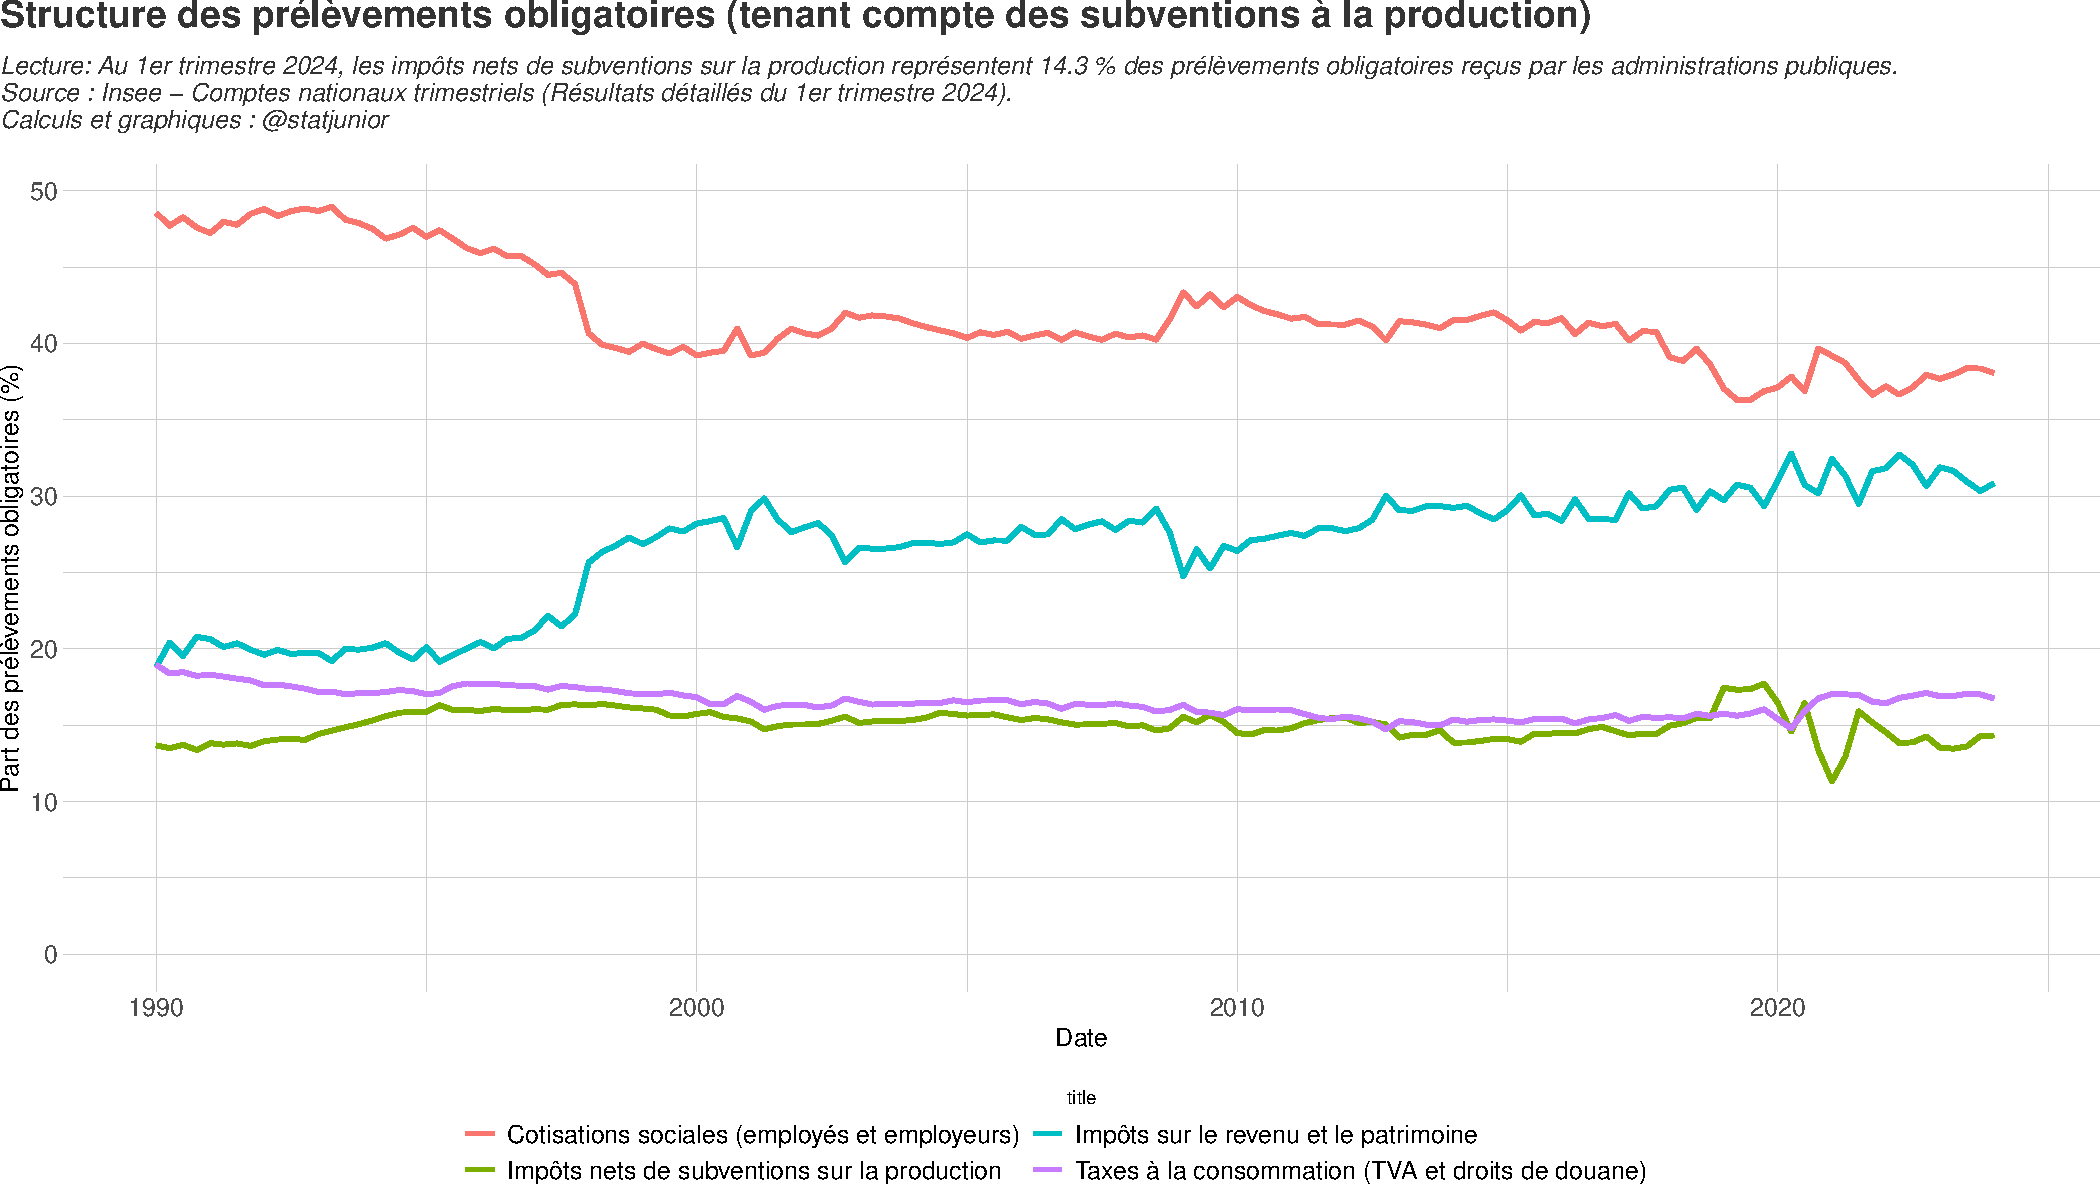
\includegraphics[keepaspectratio]{rapport_pdf_csi_files/figure-latex/unnamed-chunk-11-1.pdf}}

\subsection{Elasticité des recettes fiscales (en glissement
annuel)}\label{elasticituxe9-des-recettes-fiscales-en-glissement-annuel}

\pandocbounded{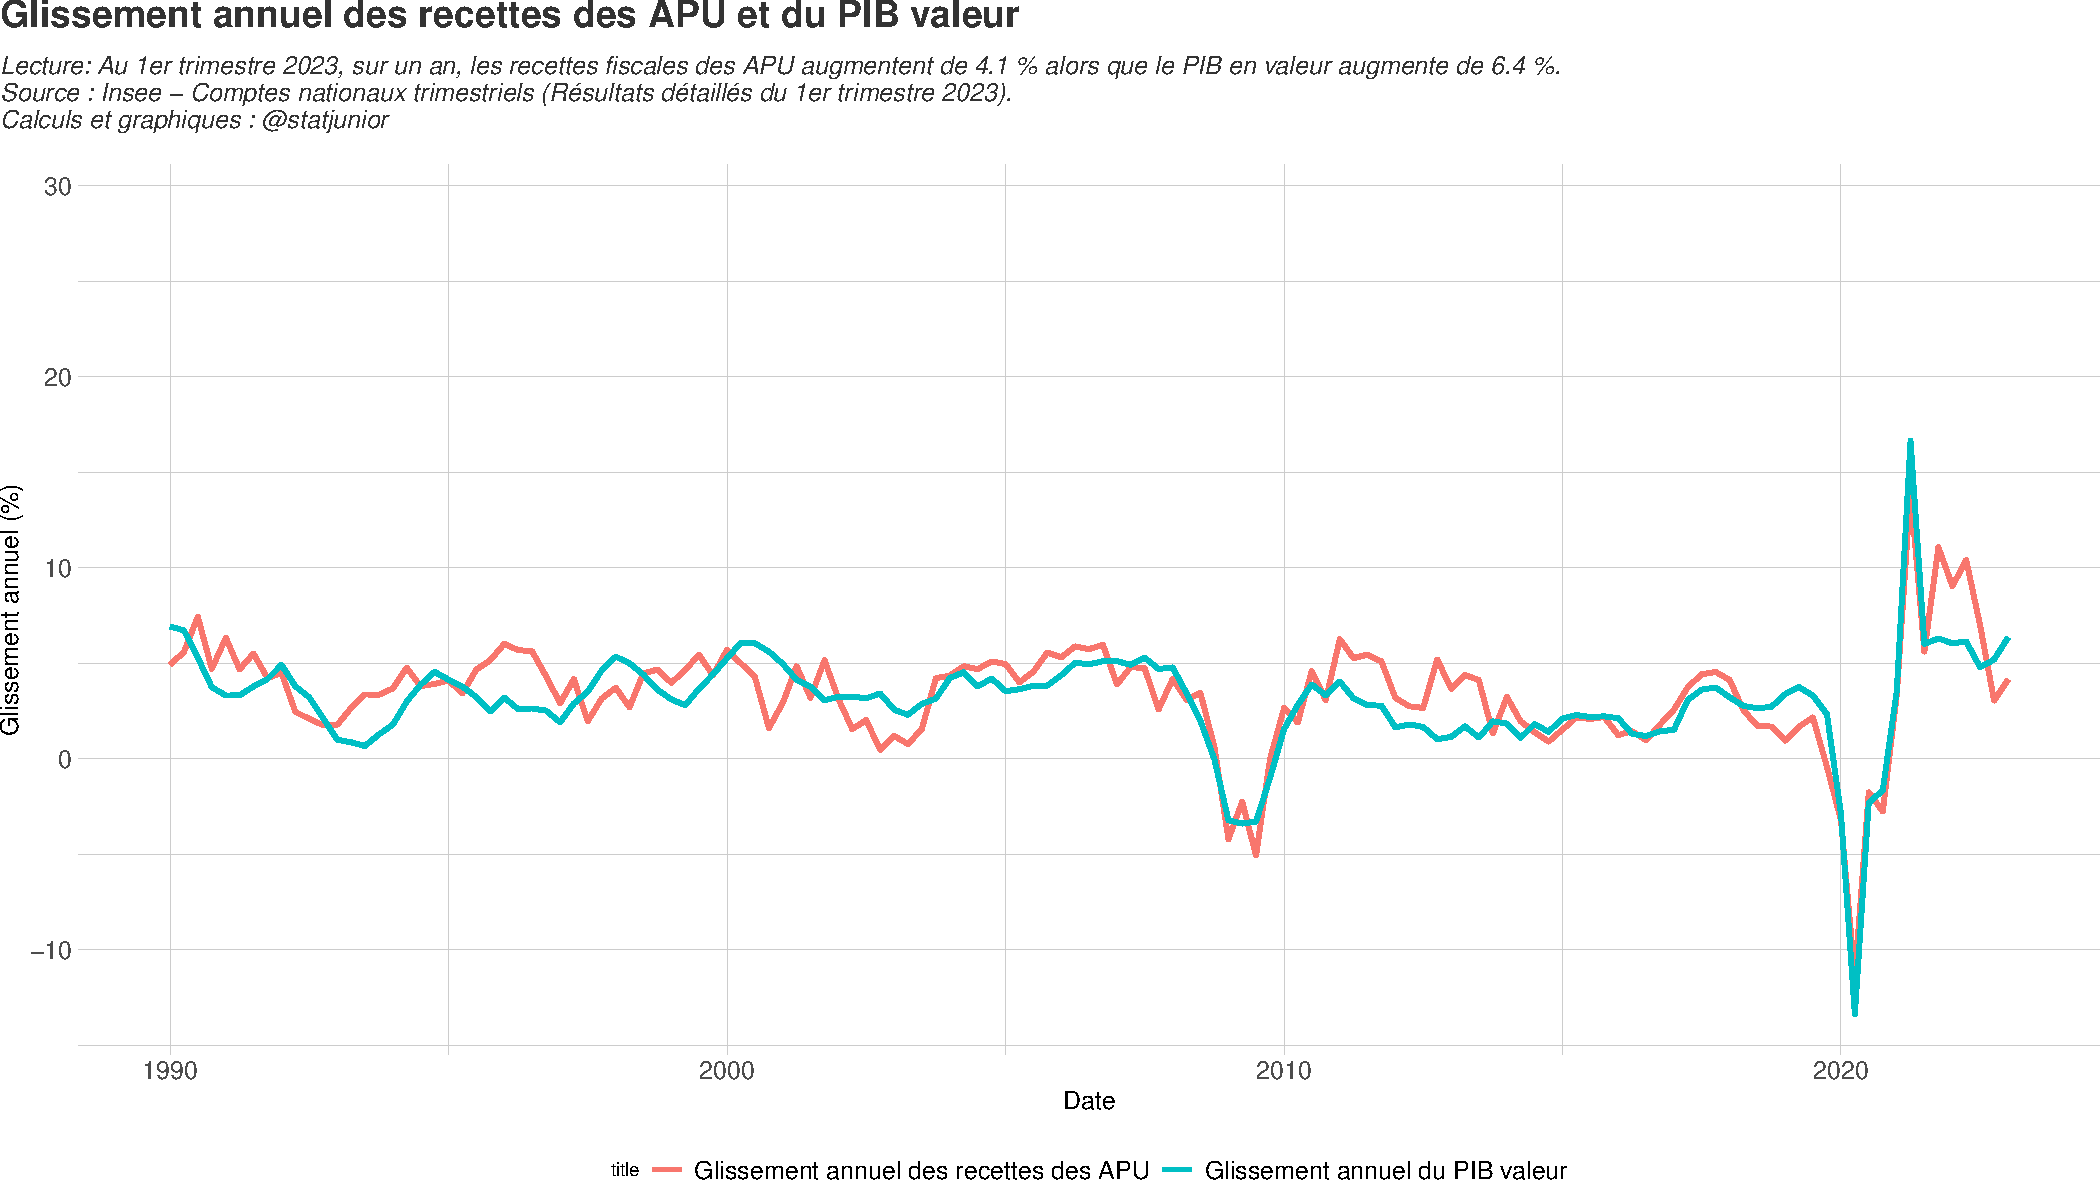
\includegraphics[keepaspectratio]{rapport_pdf_csi_files/figure-latex/unnamed-chunk-12-1.pdf}}
\pandocbounded{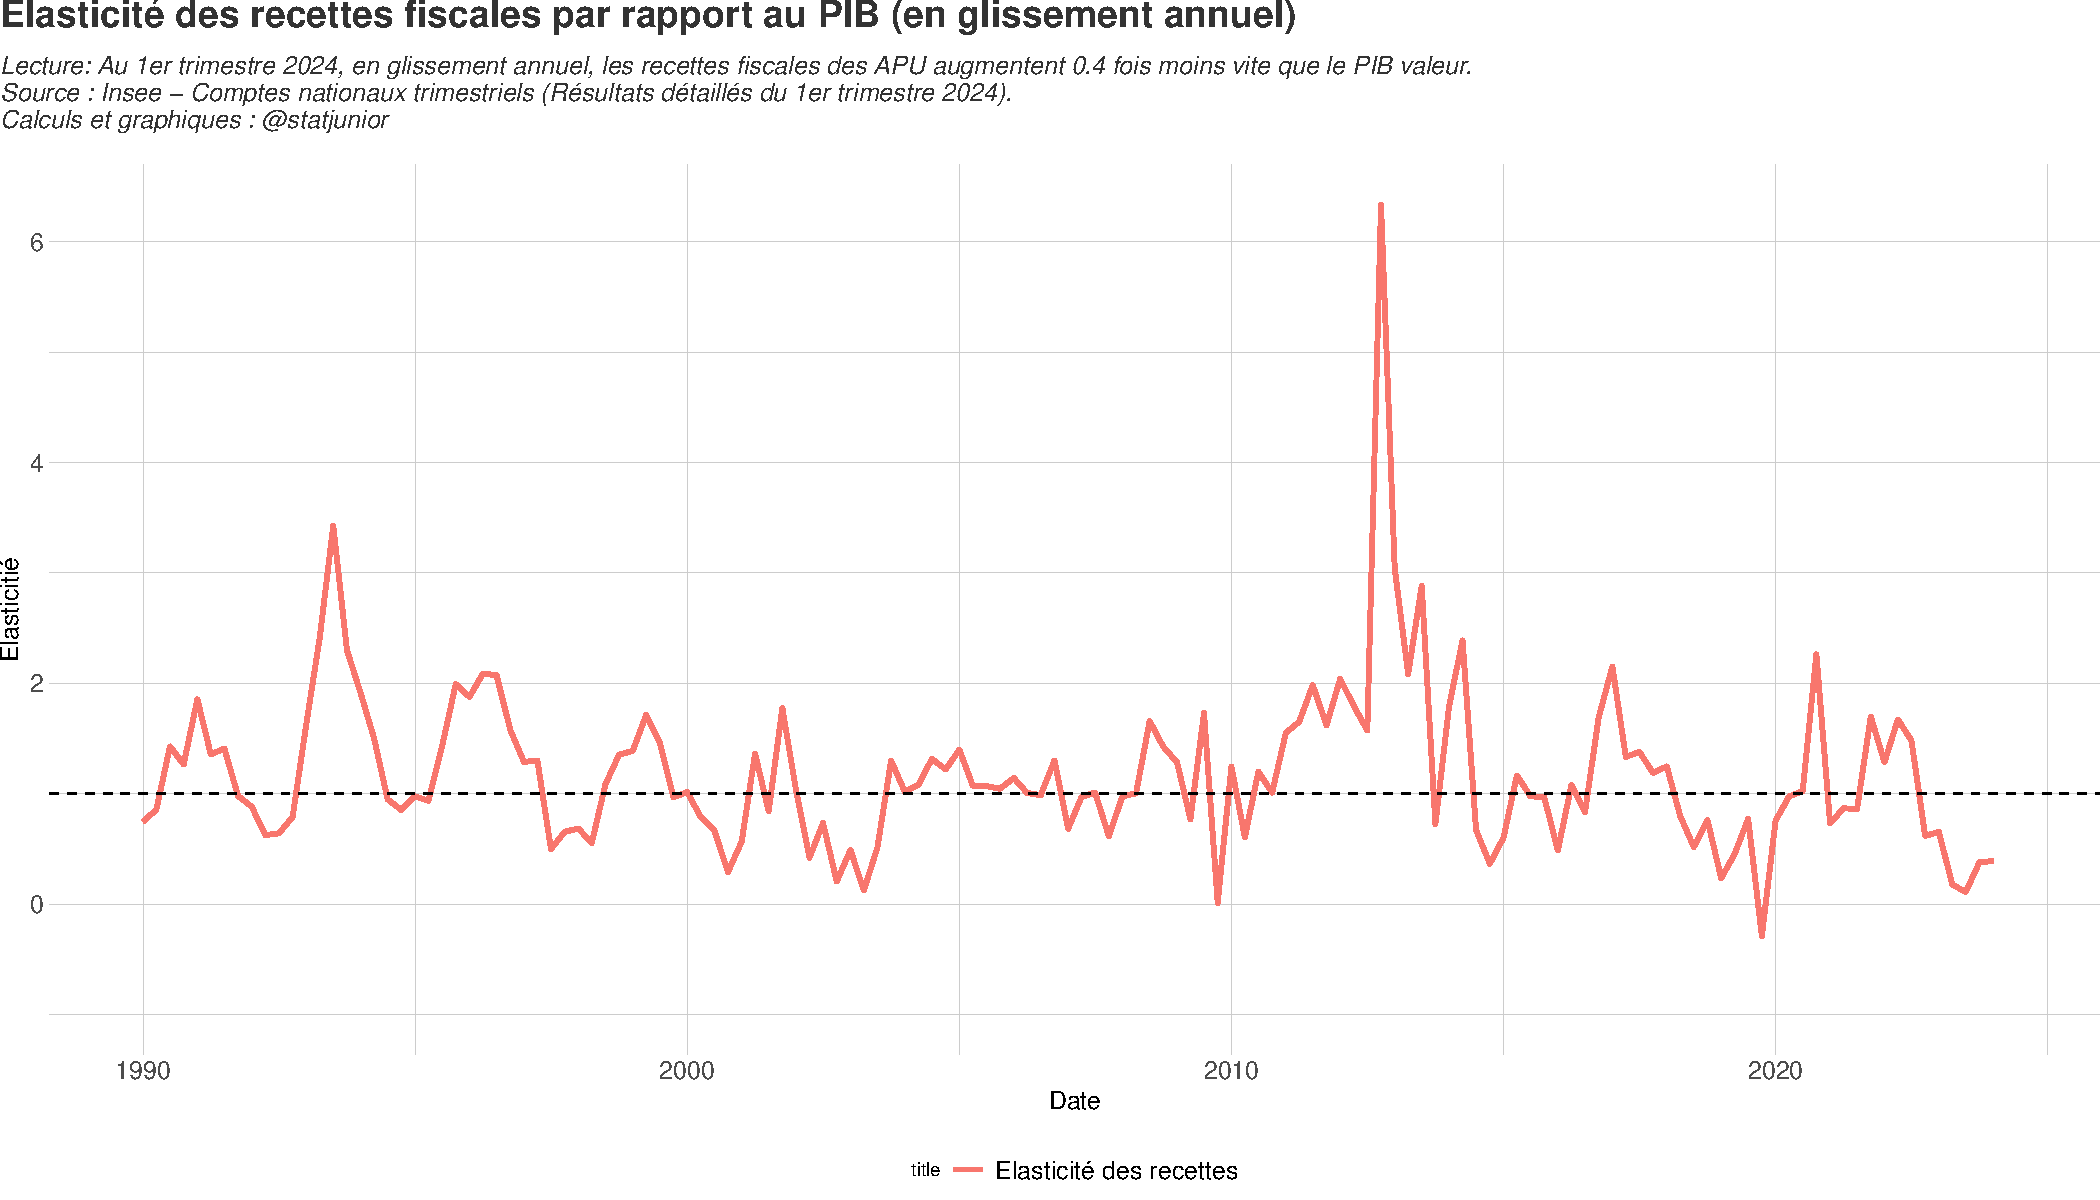
\includegraphics[keepaspectratio]{rapport_pdf_csi_files/figure-latex/unnamed-chunk-13-1.pdf}}

\subsection{Dyamisme des différentes recettes fiscales en glissement
annuel}\label{dyamisme-des-diffuxe9rentes-recettes-fiscales-en-glissement-annuel}

\pandocbounded{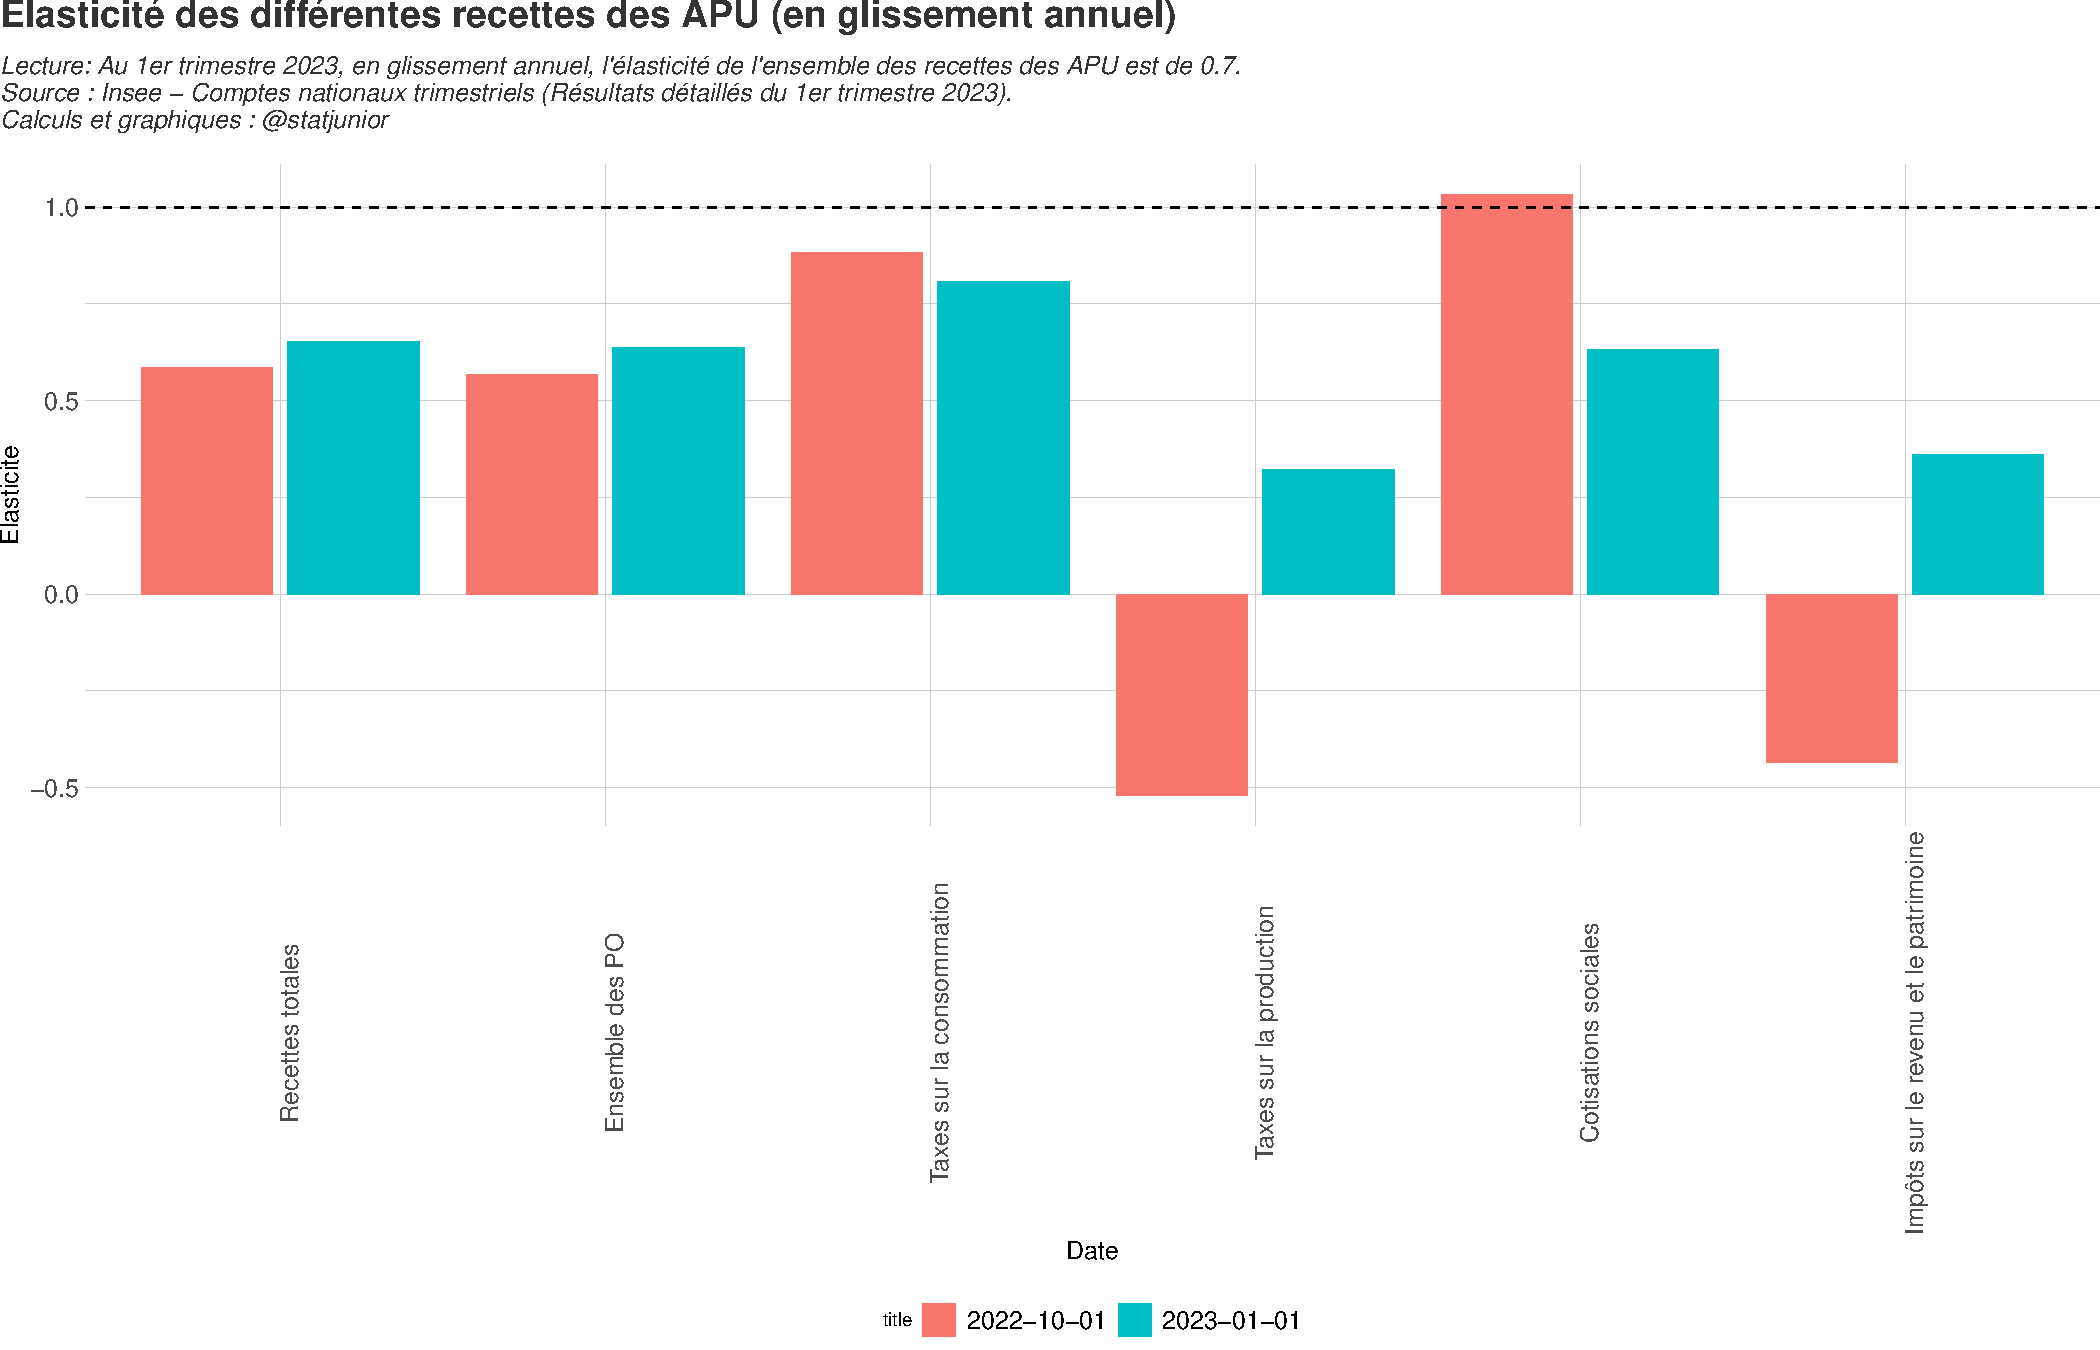
\includegraphics[keepaspectratio]{rapport_pdf_csi_files/figure-latex/unnamed-chunk-14-1.pdf}}

\subsection{Décomposition de la dépense publique par
fonctions}\label{duxe9composition-de-la-duxe9pense-publique-par-fonctions}

\pandocbounded{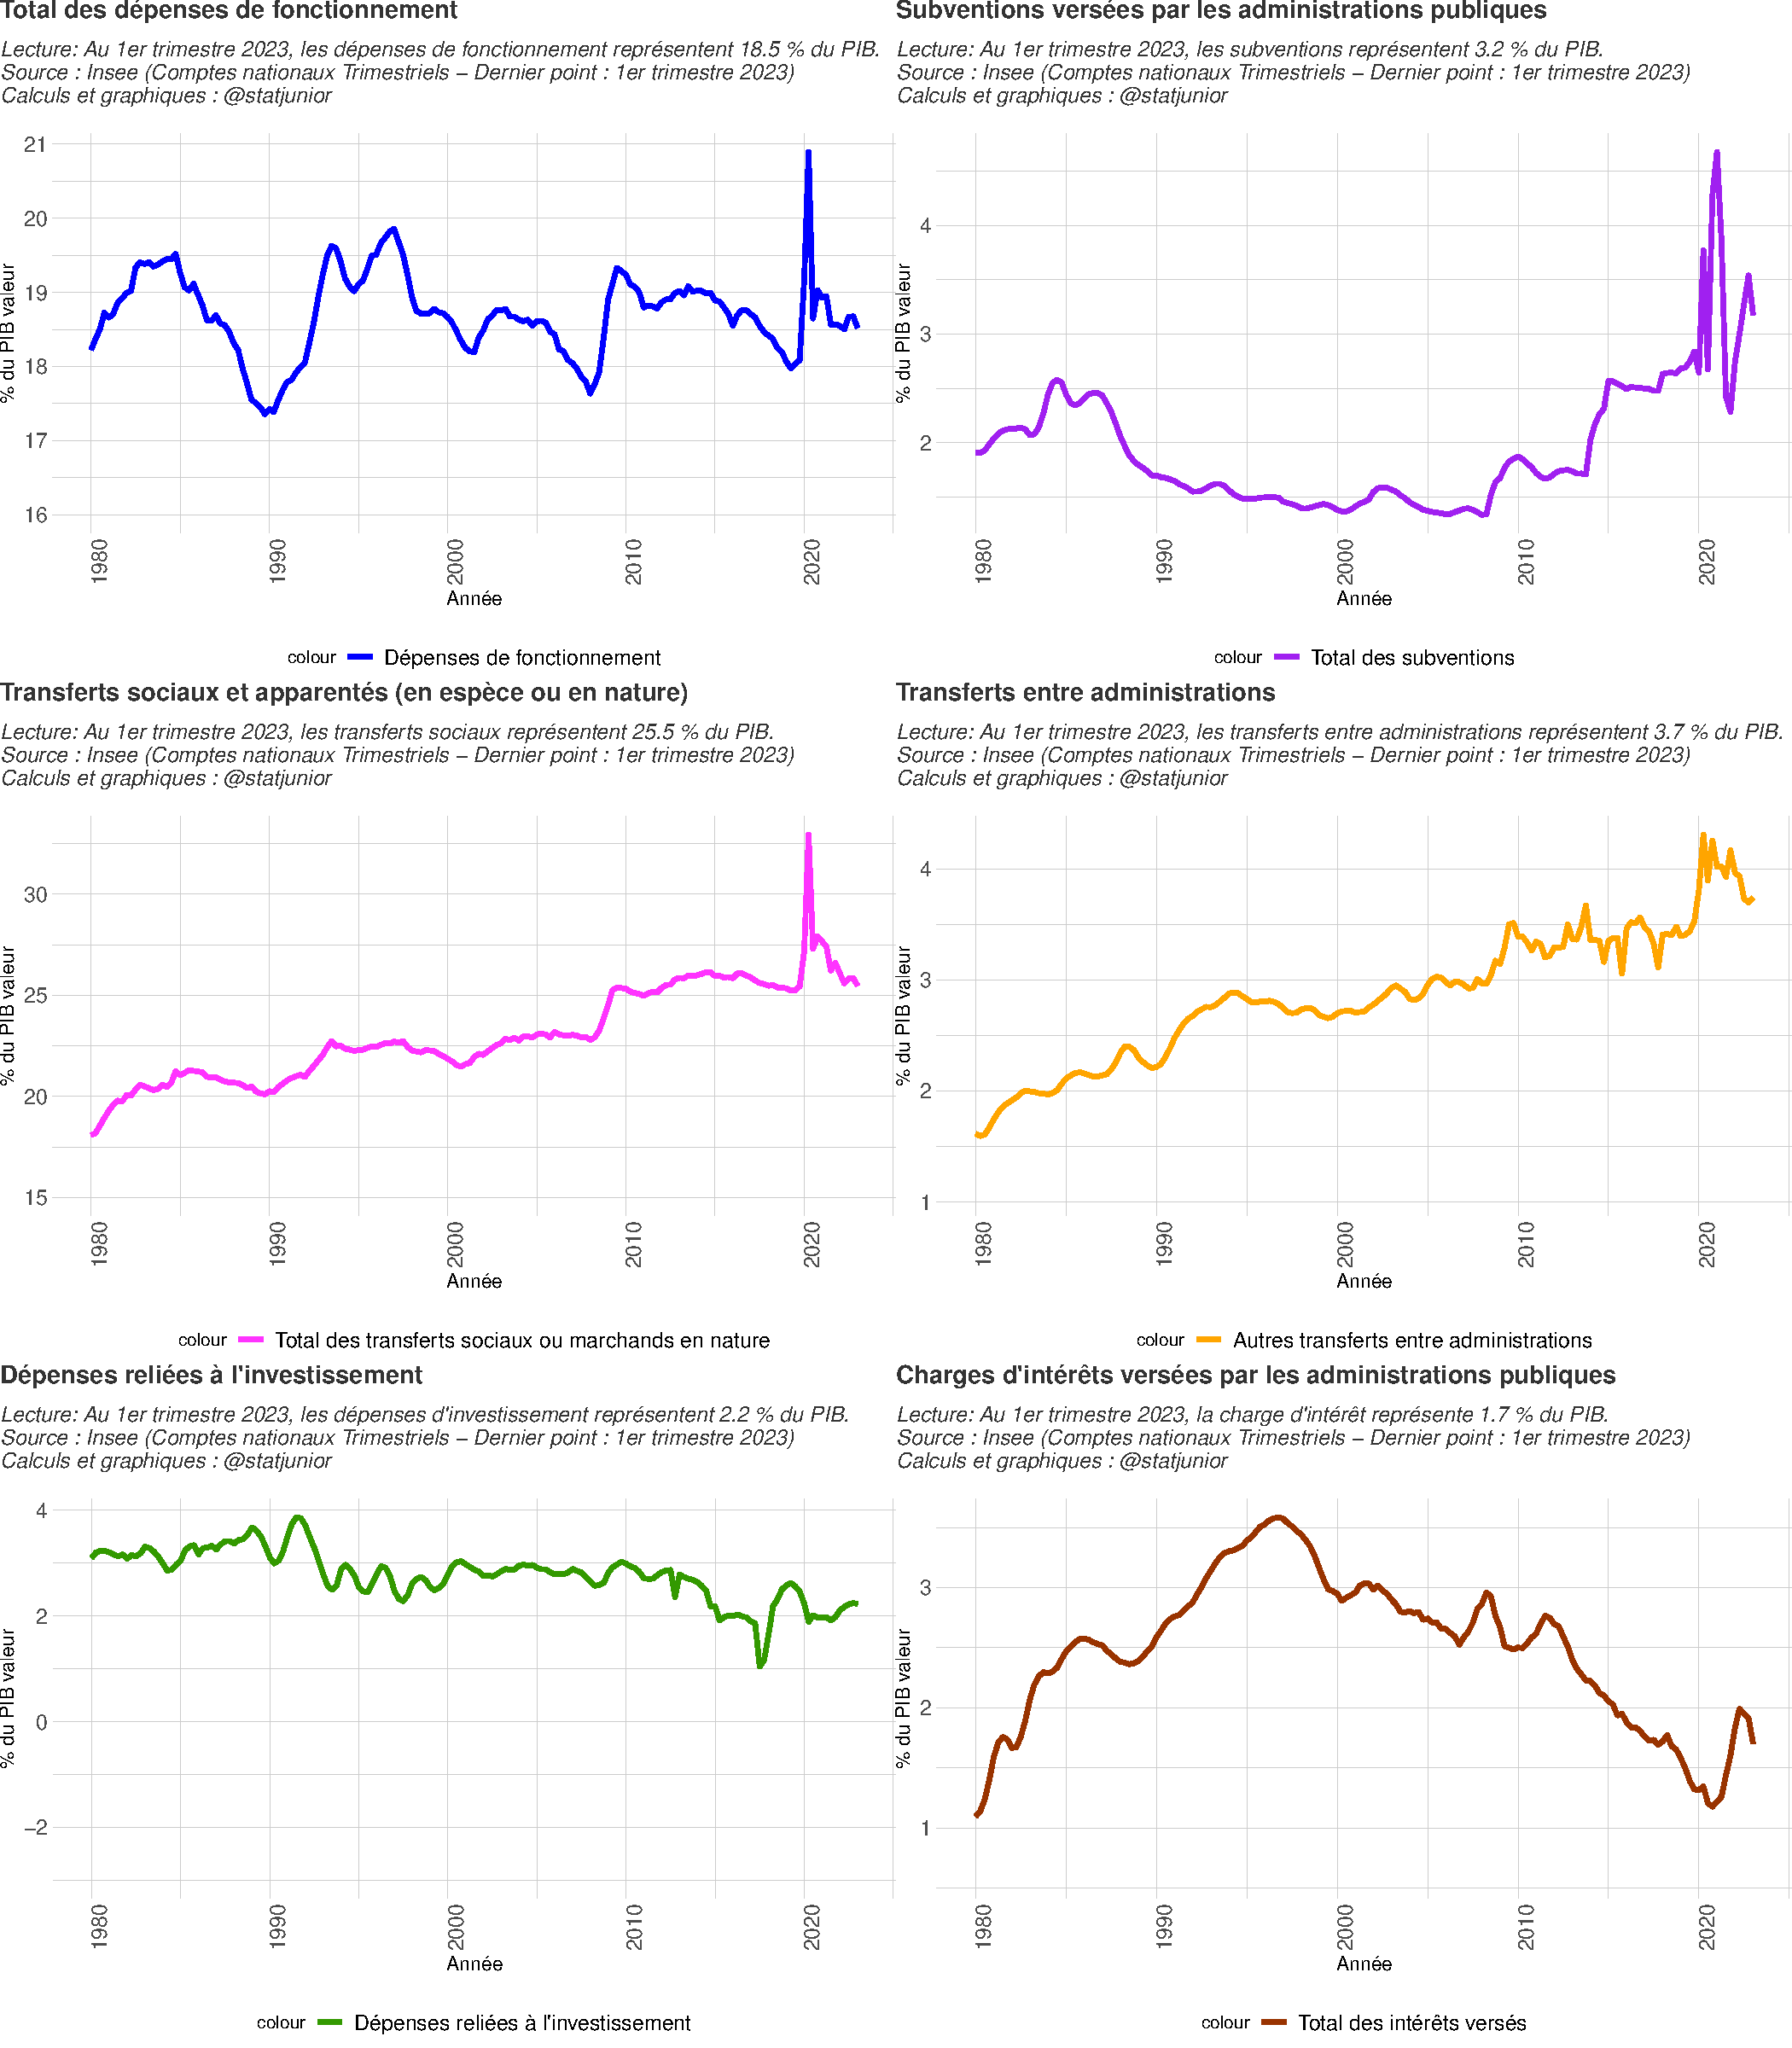
\includegraphics[keepaspectratio]{rapport_pdf_csi_files/figure-latex/unnamed-chunk-15-1.pdf}}

\subsection{Taux de déficit public des APU (avec et hors charge
d'intérêt)}\label{taux-de-duxe9ficit-public-des-apu-avec-et-hors-charge-dintuxe9ruxeat}

\pandocbounded{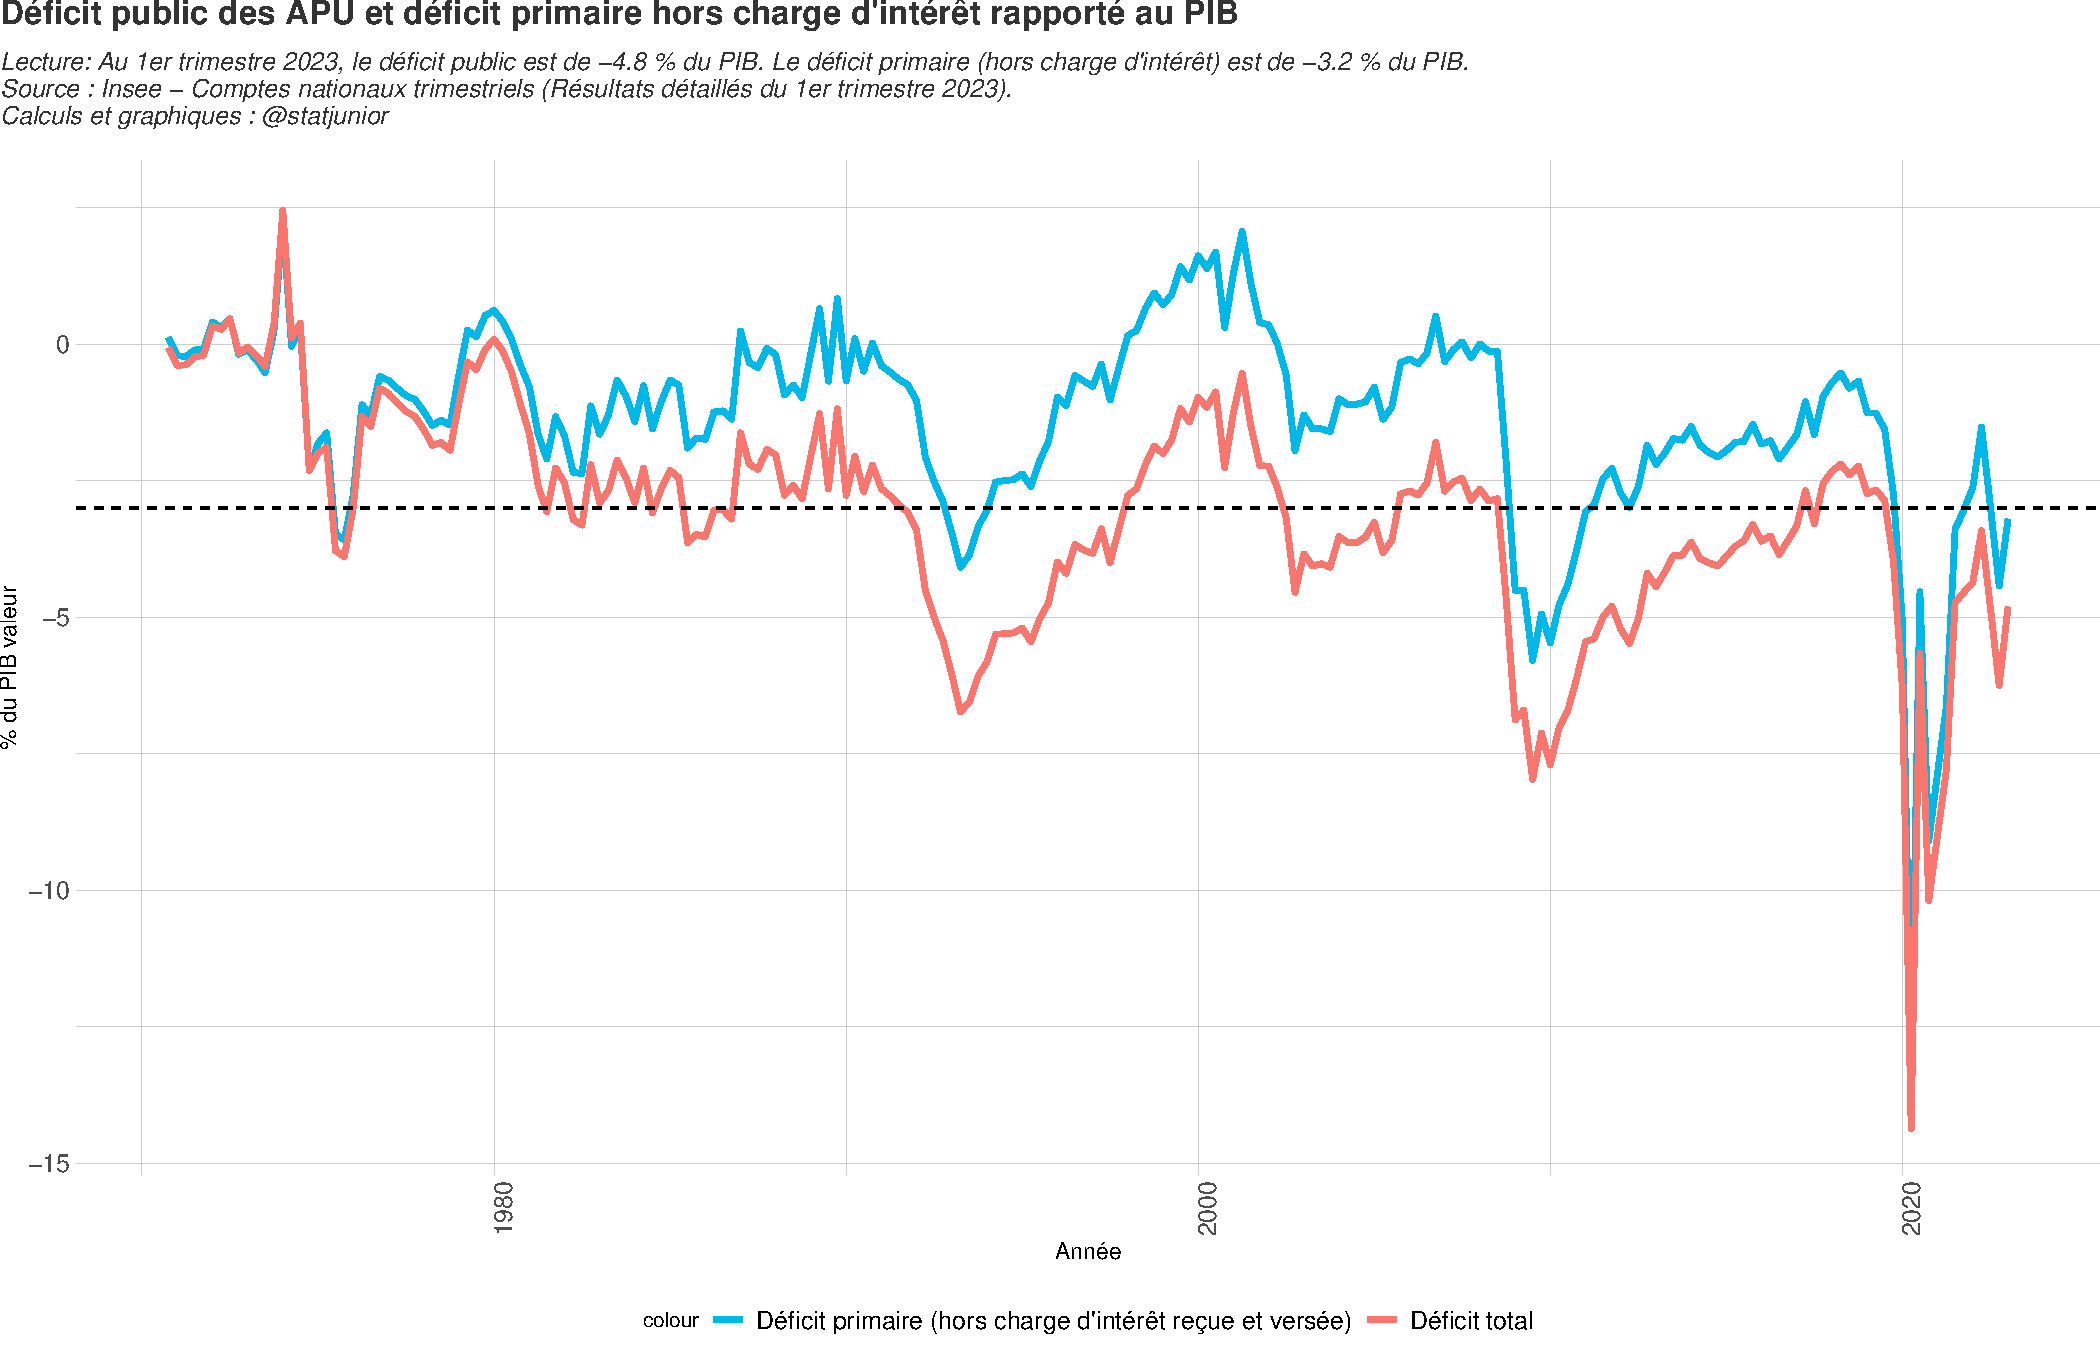
\includegraphics[keepaspectratio]{rapport_pdf_csi_files/figure-latex/unnamed-chunk-16-1.pdf}}

\subsection{Charge d'intérêt nette (versée - reçue) des administrations
publiques}\label{charge-dintuxe9ruxeat-nette-versuxe9e---reuxe7ue-des-administrations-publiques}

\pandocbounded{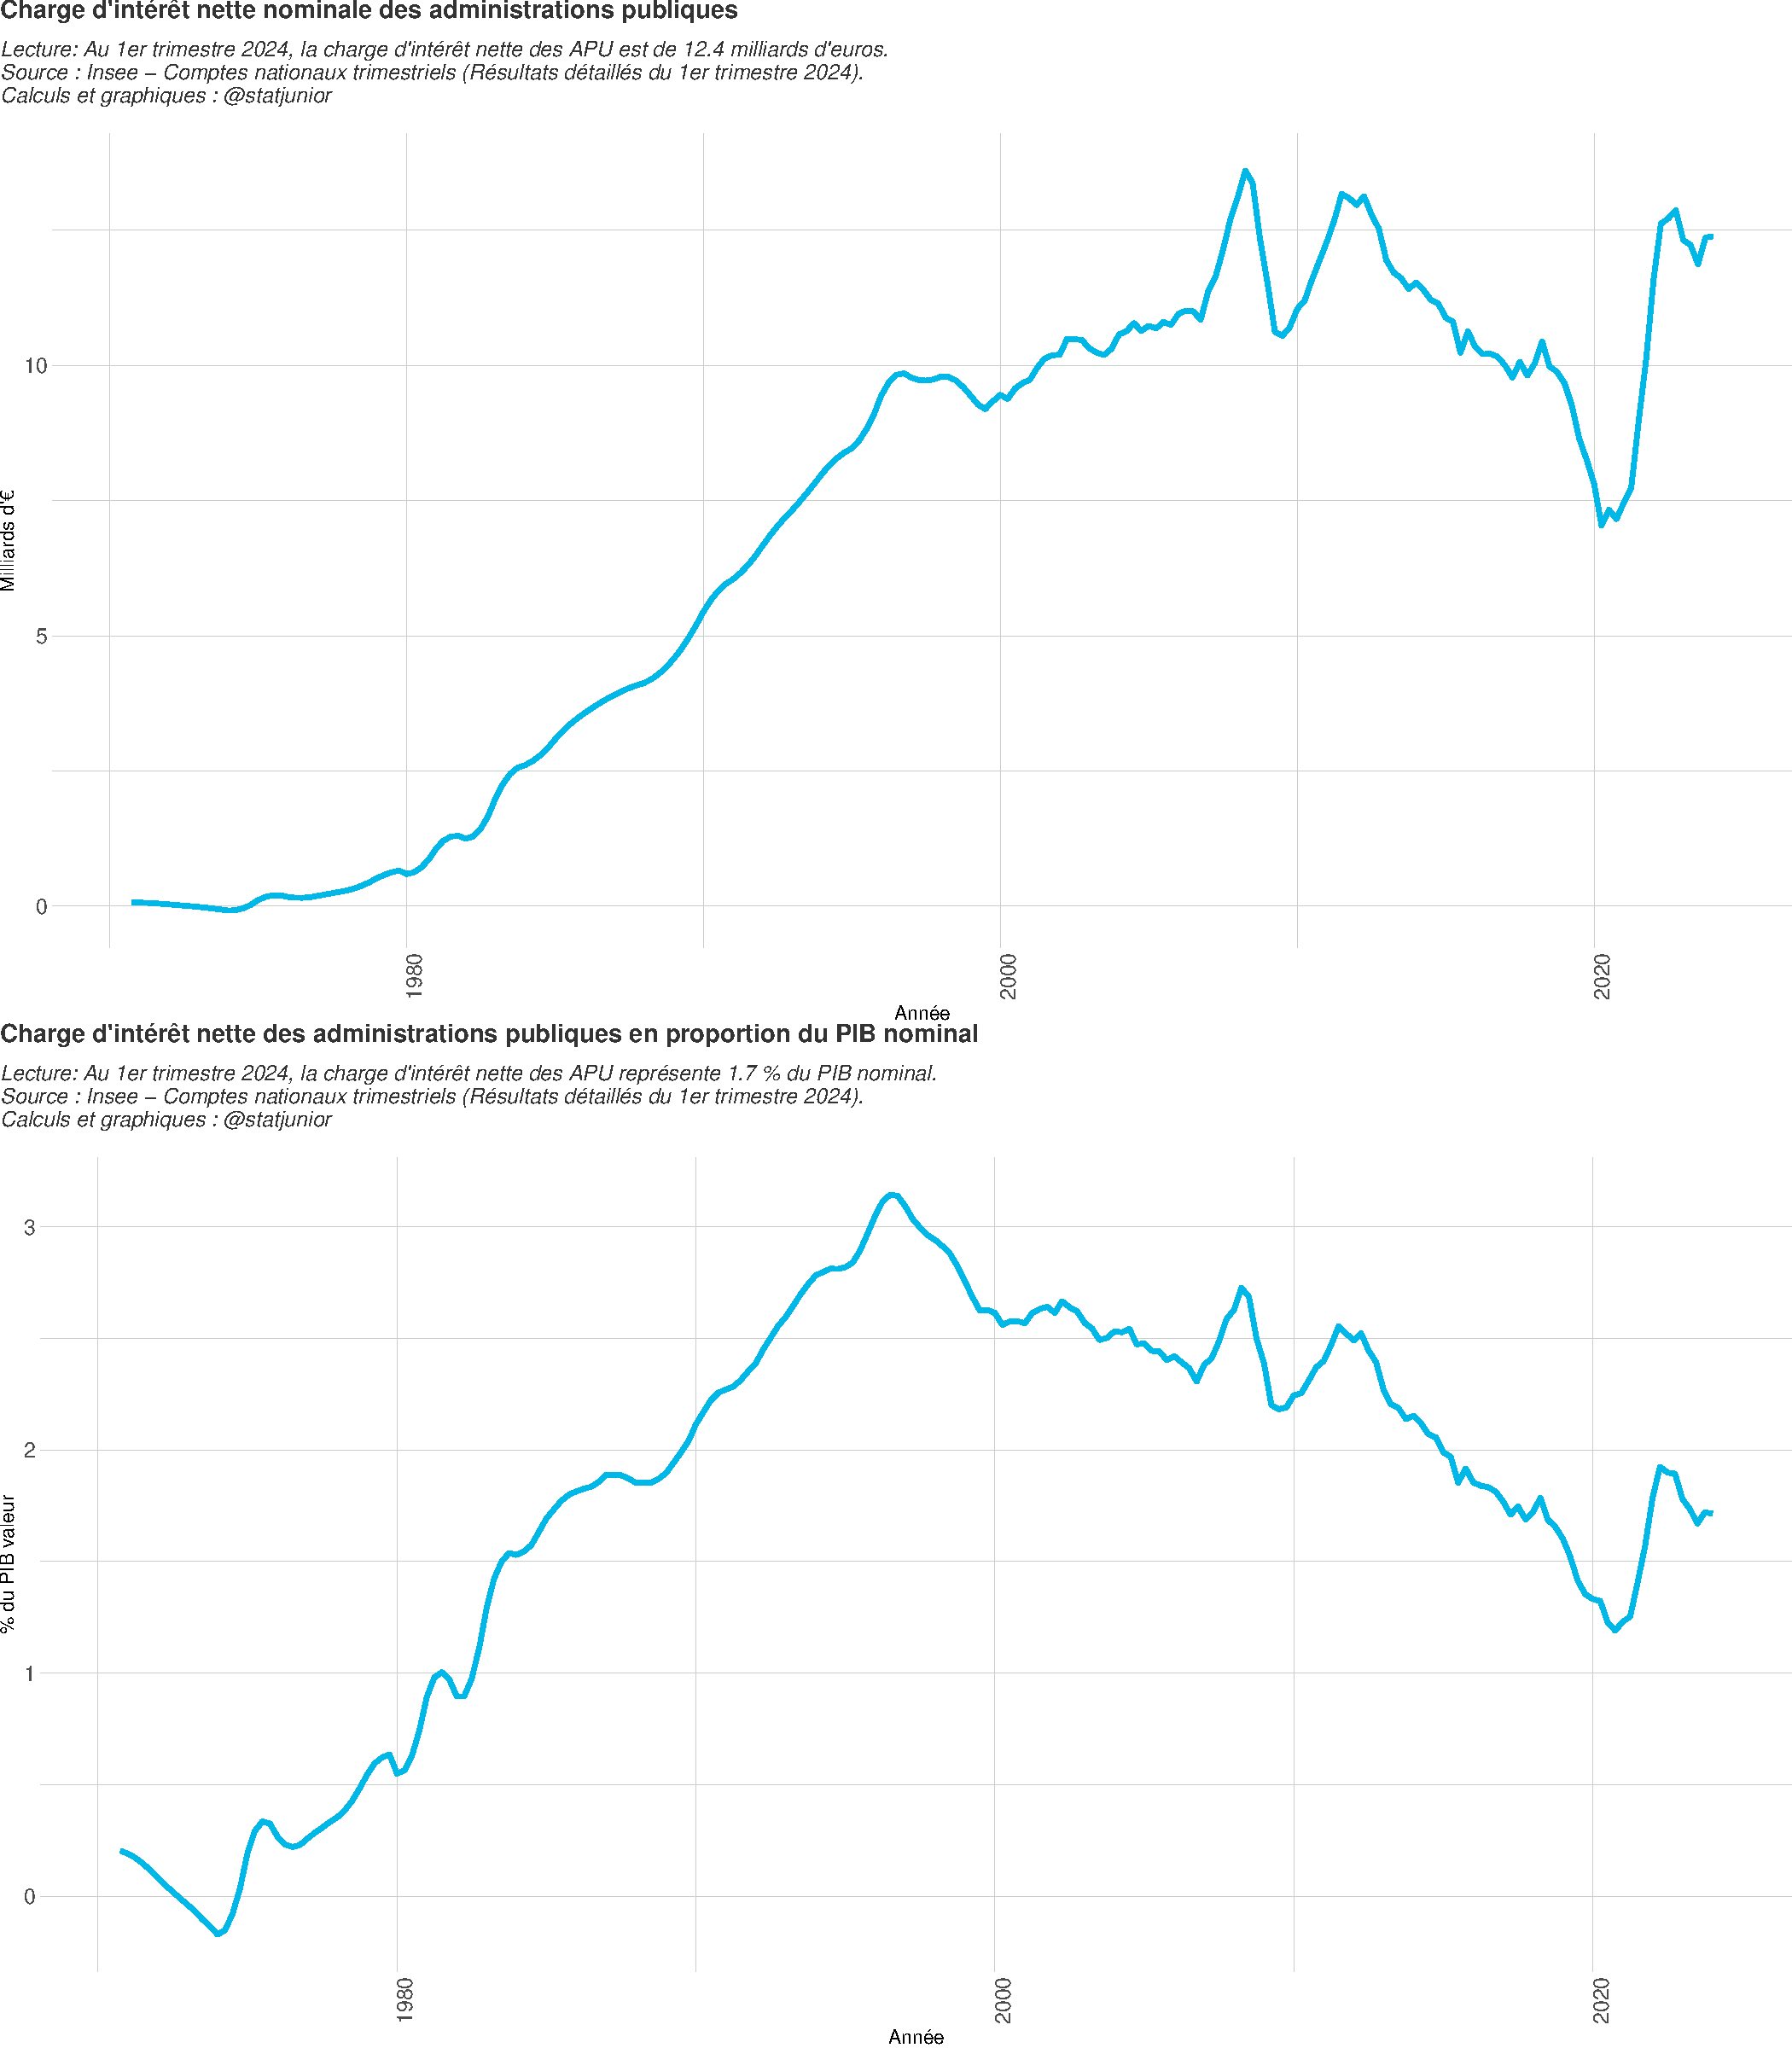
\includegraphics[keepaspectratio]{rapport_pdf_csi_files/figure-latex/unnamed-chunk-17-1.pdf}}

\newpage

\section{Capacité ou Besoin de financement vis-à-vis du Reste du
monde}\label{capacituxe9-ou-besoin-de-financement-vis-uxe0-vis-du-reste-du-monde}

\pandocbounded{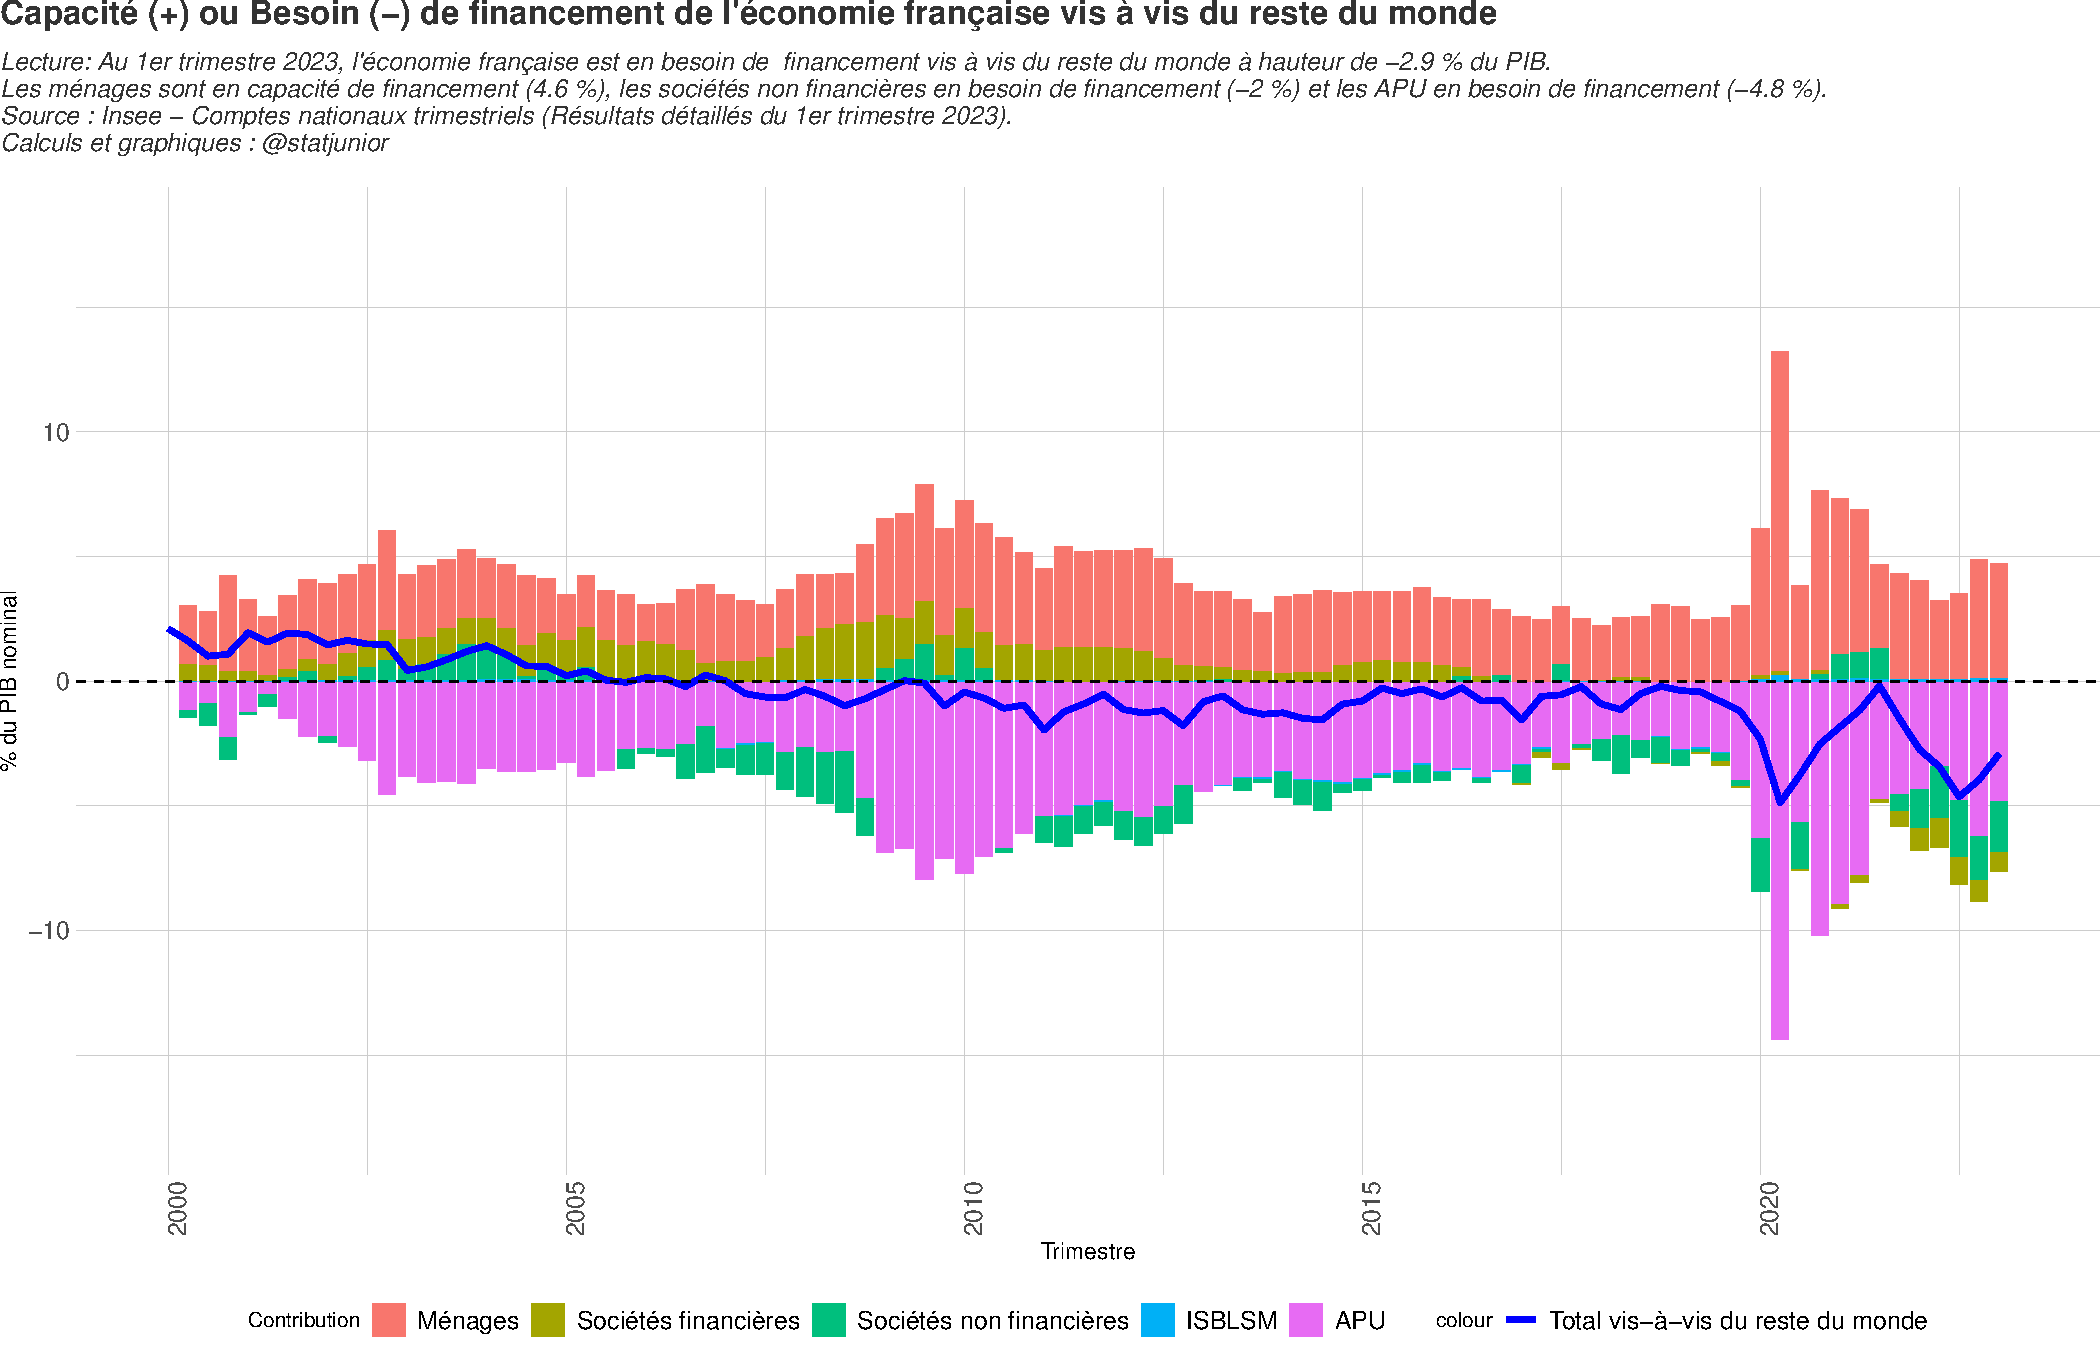
\includegraphics[keepaspectratio]{rapport_pdf_csi_files/figure-latex/unnamed-chunk-18-1.pdf}}

\end{document}
